\documentclass{beamer}
\usetheme{Madrid}
\usecolortheme{default}
\usepackage[T1]{fontenc}
\usepackage[french]{babel}
\usepackage{graphicx}
\usepackage{amsmath}
\usepackage{amssymb}
\usepackage{mathrsfs}
\usepackage{xcolor}
\usepackage{empheq}

% Ajouter le plan en haut
\useoutertheme{infolines}
\setbeamertemplate{headline}{
	\begin{beamercolorbox}[ht=2.25ex,dp=3.75ex]{section in head/foot}
		\insertnavigation{\paperwidth}
\end{beamercolorbox}}

\title[]
{Atténuation des vibrations grâce à
	un amortisseur harmonique passif}

\subtitle{}

\author{Noé Bocquillon} % (optional, for multiple authors)




\date[n°20041] % (optional)
{Numéro de candidat:\\ 20041}

%\logo{\includegraphics[height=0.8cm]{logo_uoft}}

\definecolor{uoftblue}{RGB}{6,41,88}
\setbeamercolor{titlelike}{bg=uoftblue}
\setbeamerfont{title}{series=\bfseries}
\setbeamertemplate{caption}[numbered]
\begin{document}
	
	\frame{\titlepage}
	\section{Préambule}
	\begin{frame}{Préambule}
		\frametitle{Introduction}
		
		
		\begin{columns}[T]
			\begin{column}{0.45\textwidth}
				\begin{figure}
					\centering
					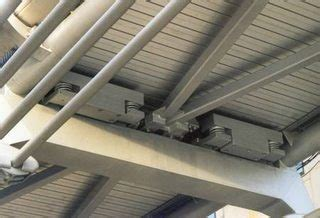
\includegraphics[width=\textwidth]{C:/Users/noebo/OneDrive/Documents/Prépa/TIPE TMD/Présentation/Photos comp/image tmd pont-min.jpg}
					\caption{Tuned mass damper sur un pont}
				\end{figure}
				
			\end{column}
			\begin{column}{0.45\textwidth}
				\begin{figure}
					\centering
					\caption{ Pendule de la tour Tapei 101 à Taiwan}
					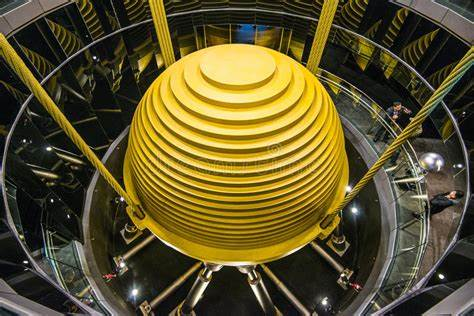
\includegraphics[width=\textwidth]{C:/Users/noebo/OneDrive/Documents/Prépa/TIPE TMD/Présentation/Photos comp/image tour tawai pendule-min.jpg}
				\end{figure}
			\end{column}
		\end{columns}
		\bigskip\small TMD = Tuned mass damper
	\end{frame}
	
	%\section{First section}
	\begin{frame}{Préambule}
		\frametitle{Objectifs}
		\underline{Problématique:} Quelle est l'influence du Tuned Mass Damper lors d'une excitation extérieure ? 
		\vspace{12pt}
		\linebreak[3]Objectifs du TIPE:
		\begin{itemize}
			\item\ Modéliser un immeuble subissant une contrainte extérieure
			\item Étudier l'influence du TMD et de ses paramètres sur l'atténuation des vibrations de la maquette
			
		\end{itemize}
		
	\end{frame}
	
	\begin{frame}{Plan}
		\begin{enumerate}
			\item\huge{Construction de la maquette et développement de l'outil de vibration} \linebreak
			\item Mise en vibration de la maquette\linebreak
			\item Élaboration d'un modèle théorique et conclusion 
		\end{enumerate}
	\end{frame}
	
	\section{Construction de la maquette}
	\begin{frame}{Construction de la maquette}
		Schéma global du système
		\begin{columns}
			\begin{column}{0.3\textwidth}
				\begin{figure}
					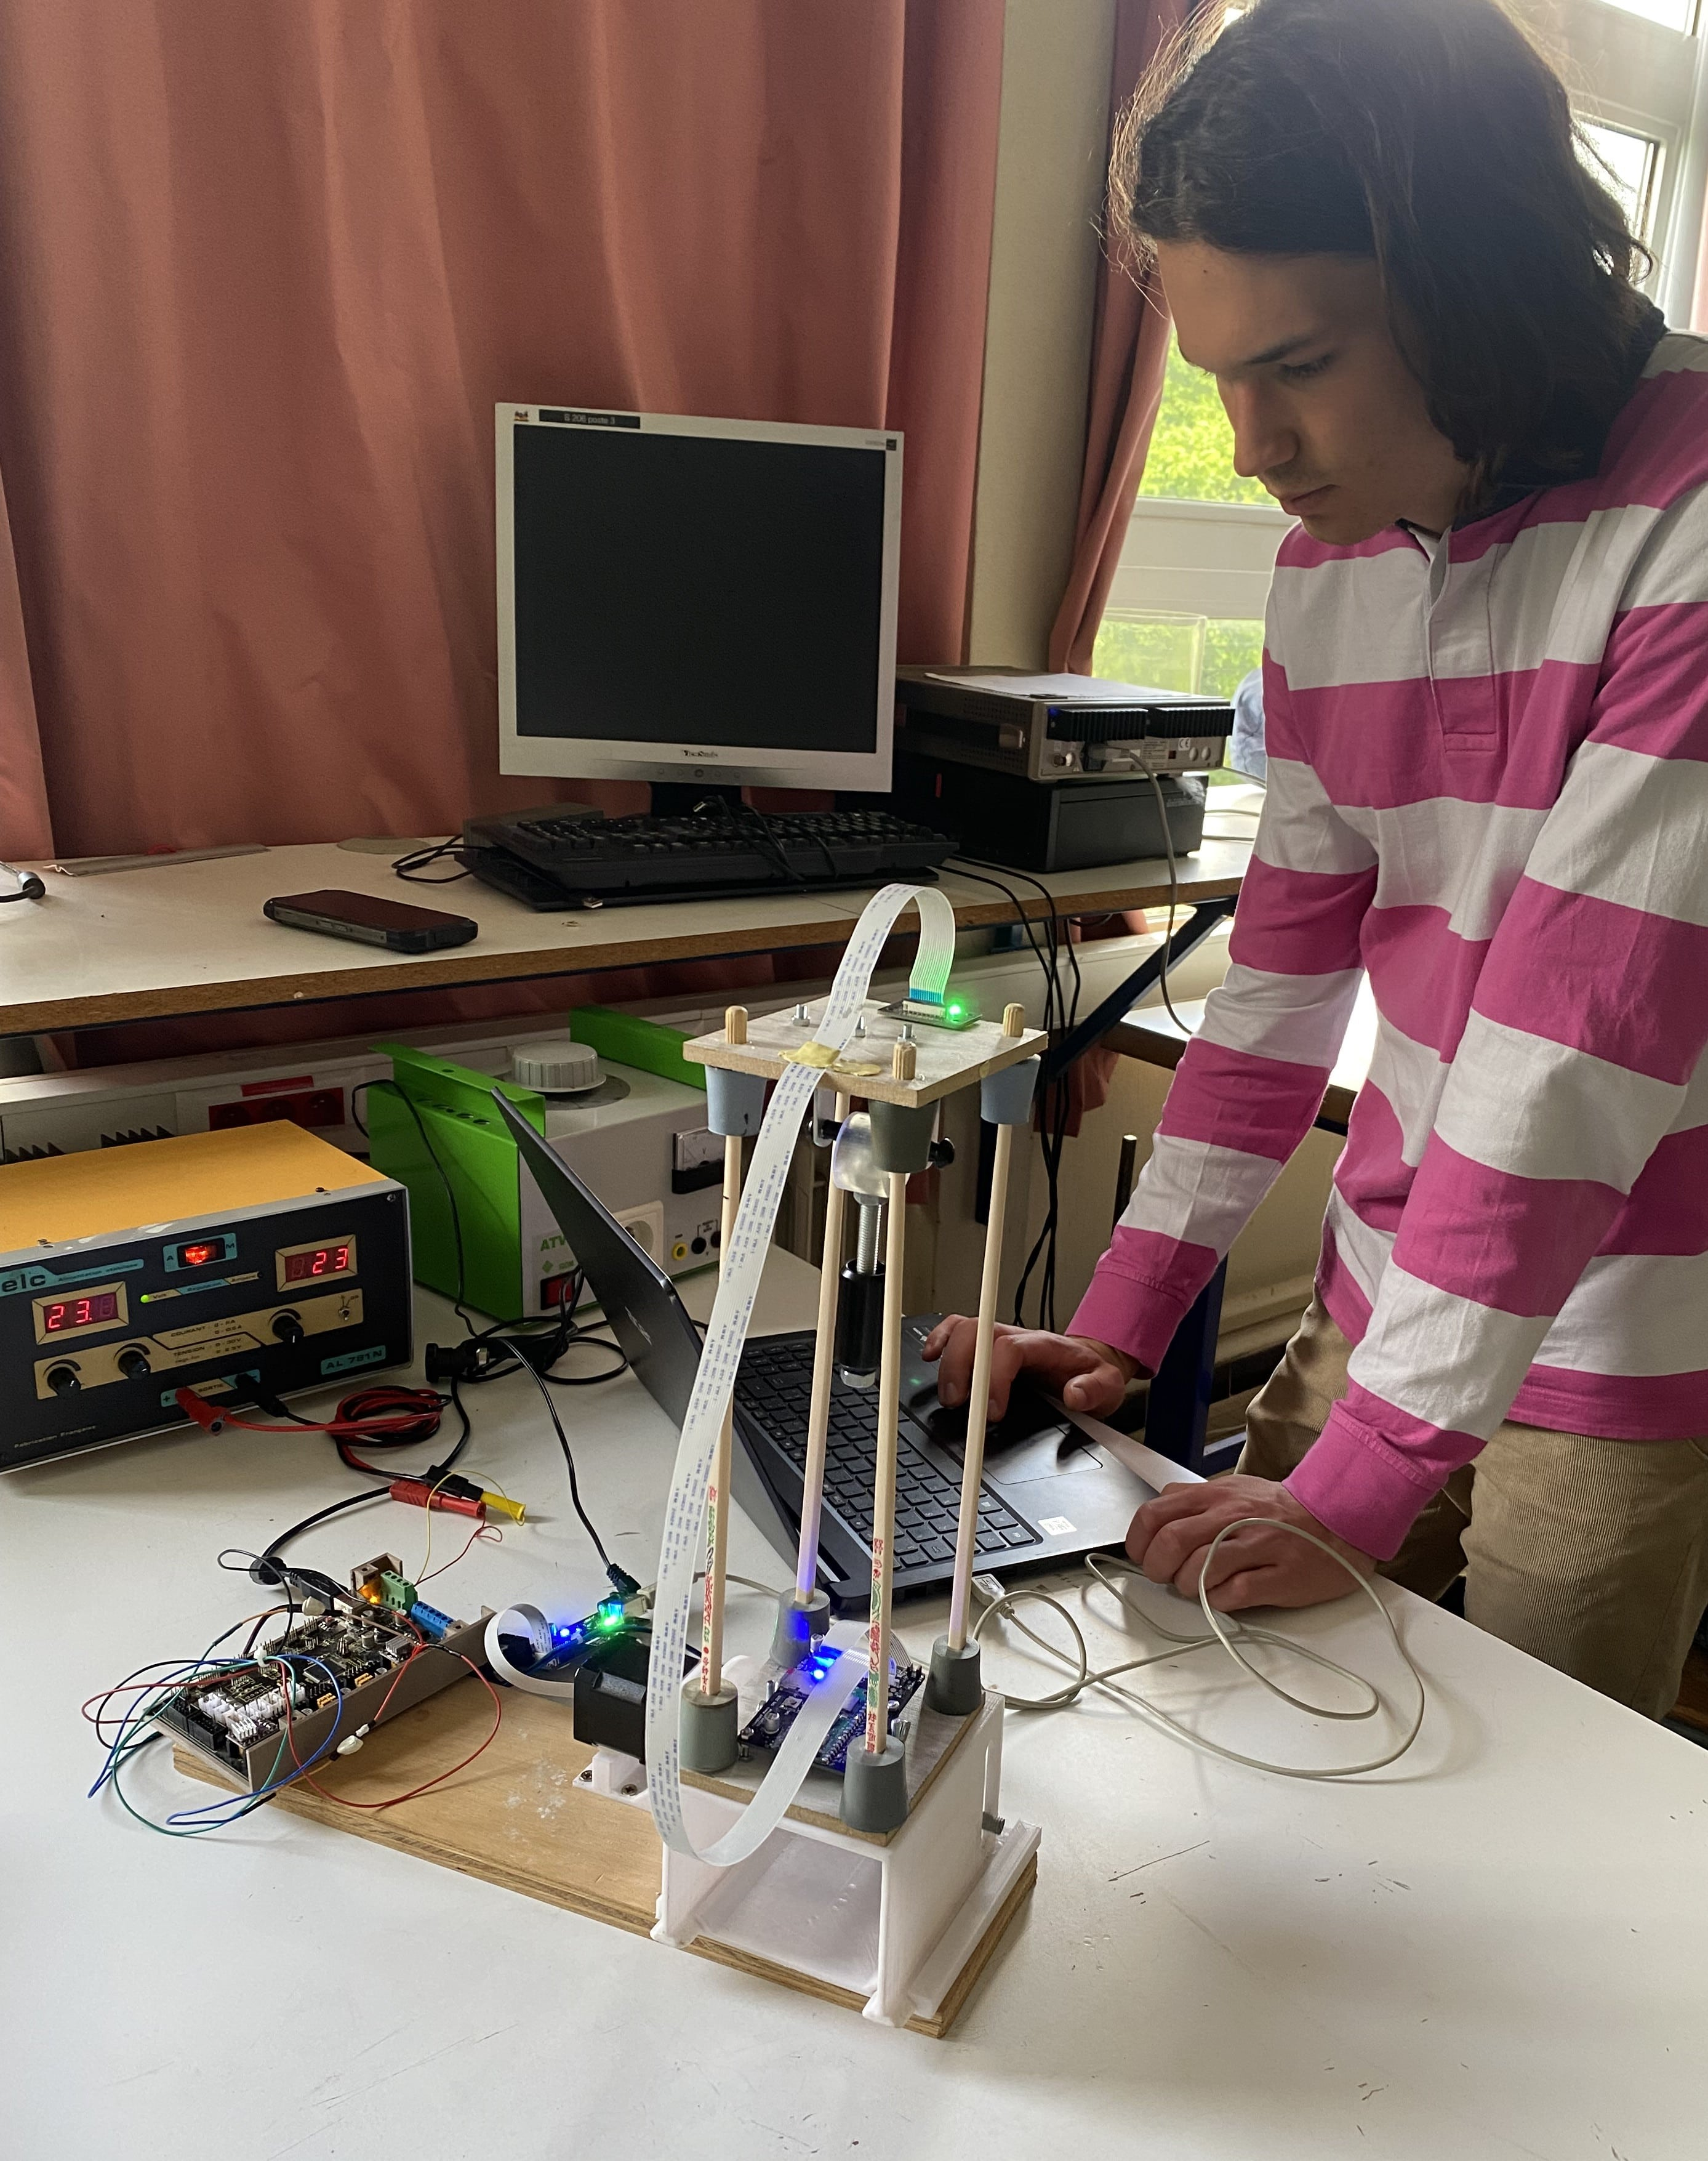
\includegraphics[width=\textwidth]{C:/Users/noebo/OneDrive/Documents/Prépa/TIPE TMD/Présentation/Photos comp/IMG_3412-min.JPG}
					\caption{Montage global}
				\end{figure}
				%Changer photo , plus global plus zoom
			\end{column}
			\begin{column}{0.3\textwidth}
			
			\begin{figure}
				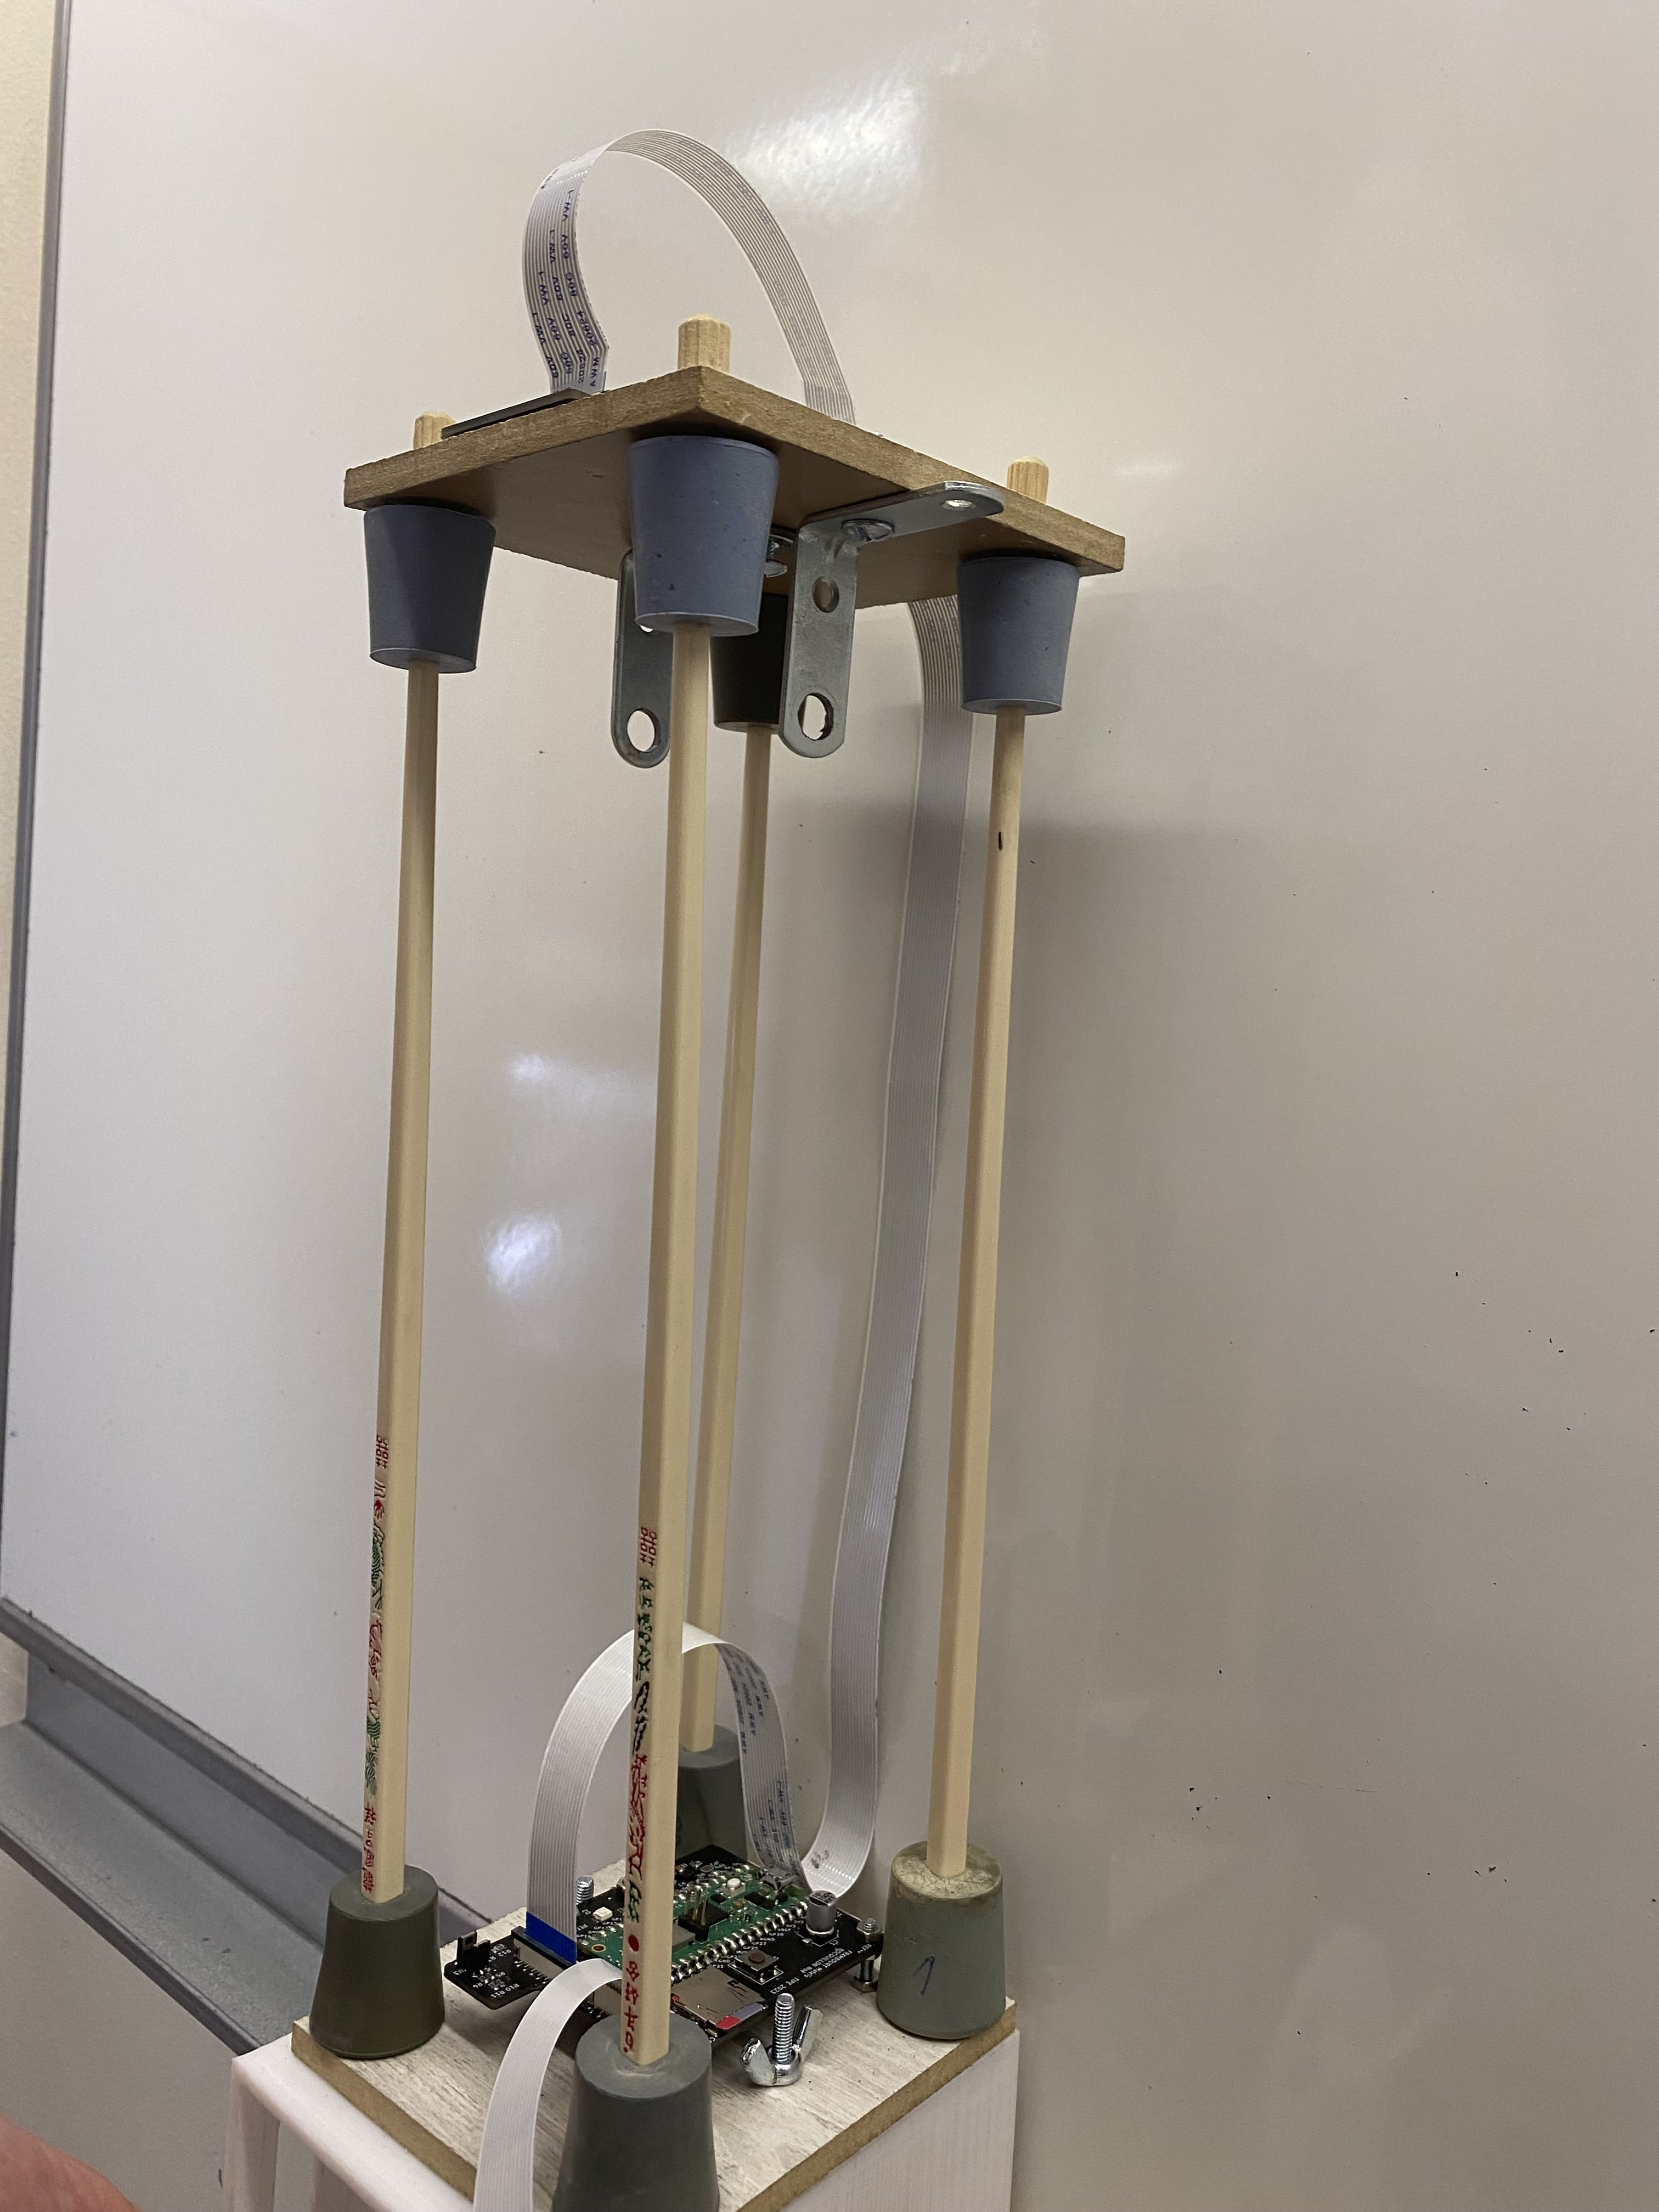
\includegraphics[width=\textwidth]{C:/Users/noebo/OneDrive/Documents/Prépa/TIPE TMD/Présentation/Photos comp/IMG_3380-min.JPG}
				\caption{Maquette de l'immeuble}
			\end{figure}
			\end{column}
	
		\begin{column}{0.2\textwidth}
				Contraintes:
		\begin{itemize}
			\item Taille
			\item Flexibilité \\
		\end{itemize}
		\end{column}
	\end{columns}
	\end{frame}


\begin{frame}{Schéma de la maquette}
	\begin{figure}
		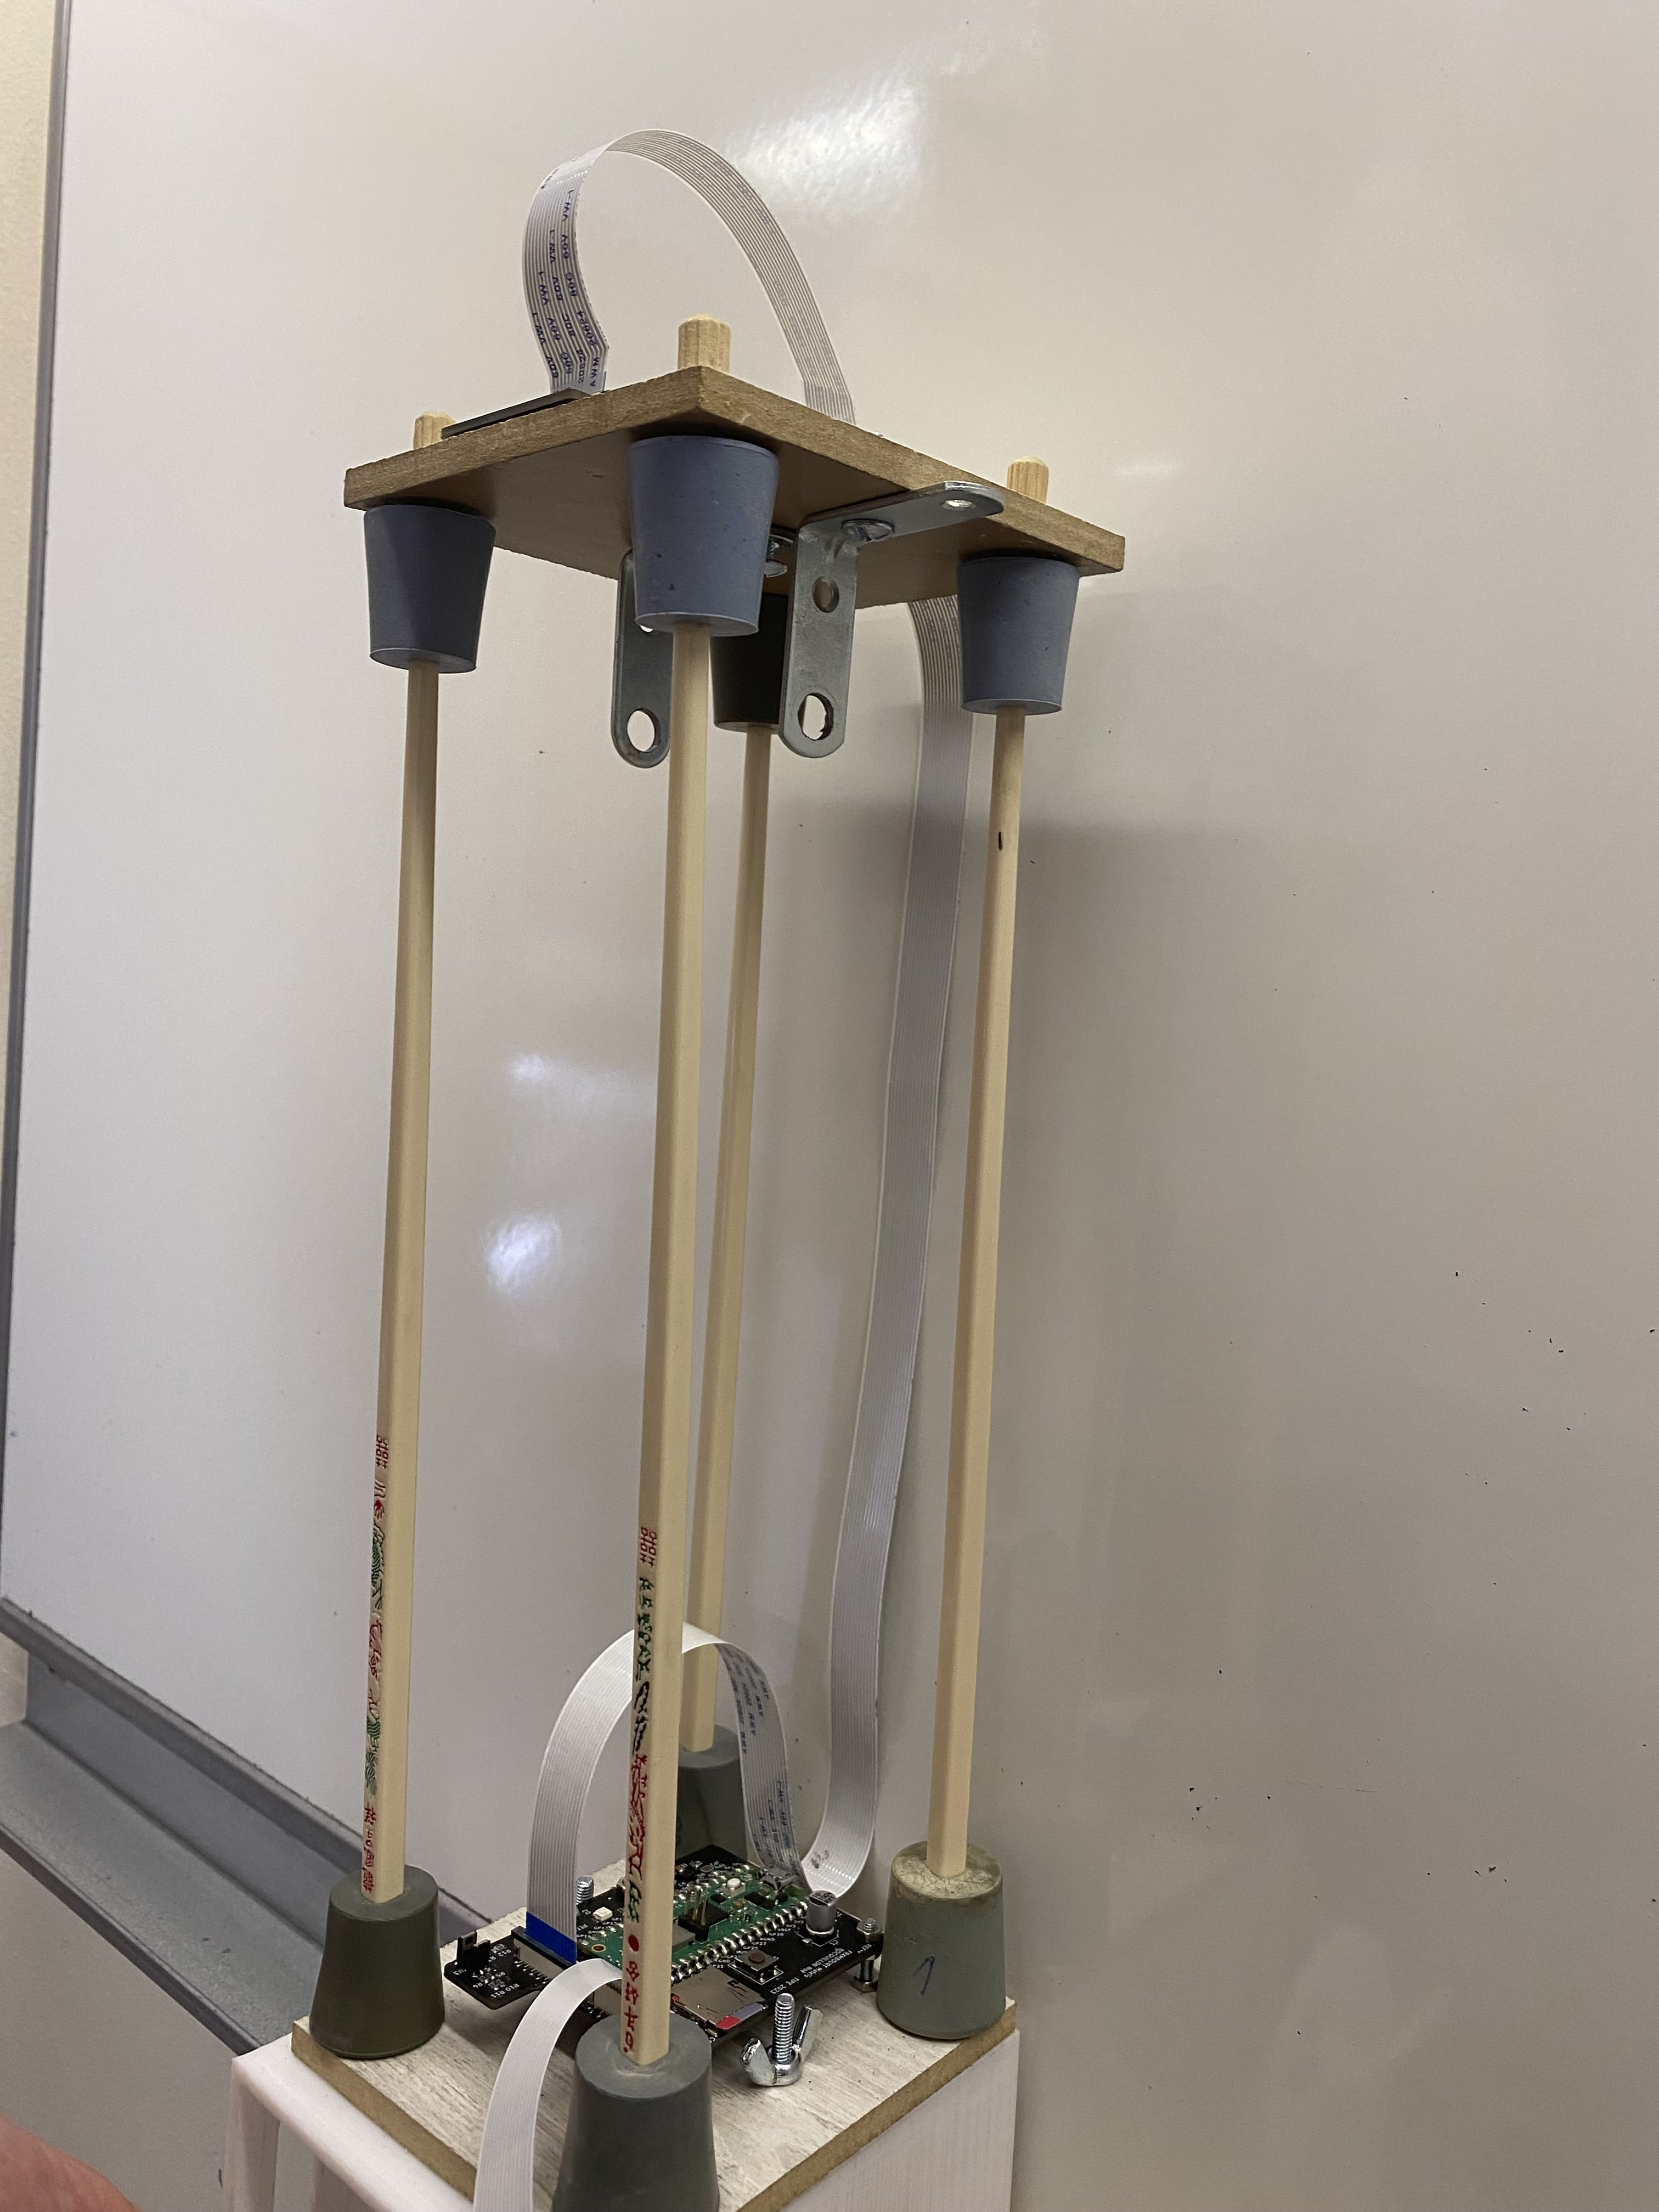
\includegraphics[width=0.3\textwidth]{C:/Users/noebo/OneDrive/Documents/Prépa/TIPE TMD/Présentation/Photos comp/IMG_3380-min.JPG}
		\caption{Schéma de la maquette de l'immeuble}
	\end{figure}
\end{frame}

	
	\begin{frame}{Construction de la maquette}
		\frametitle{Pendule}
		\begin{columns}
			Pivot d'axe:
			\begin{column}{0,45\textwidth}
				\begin{figure}
					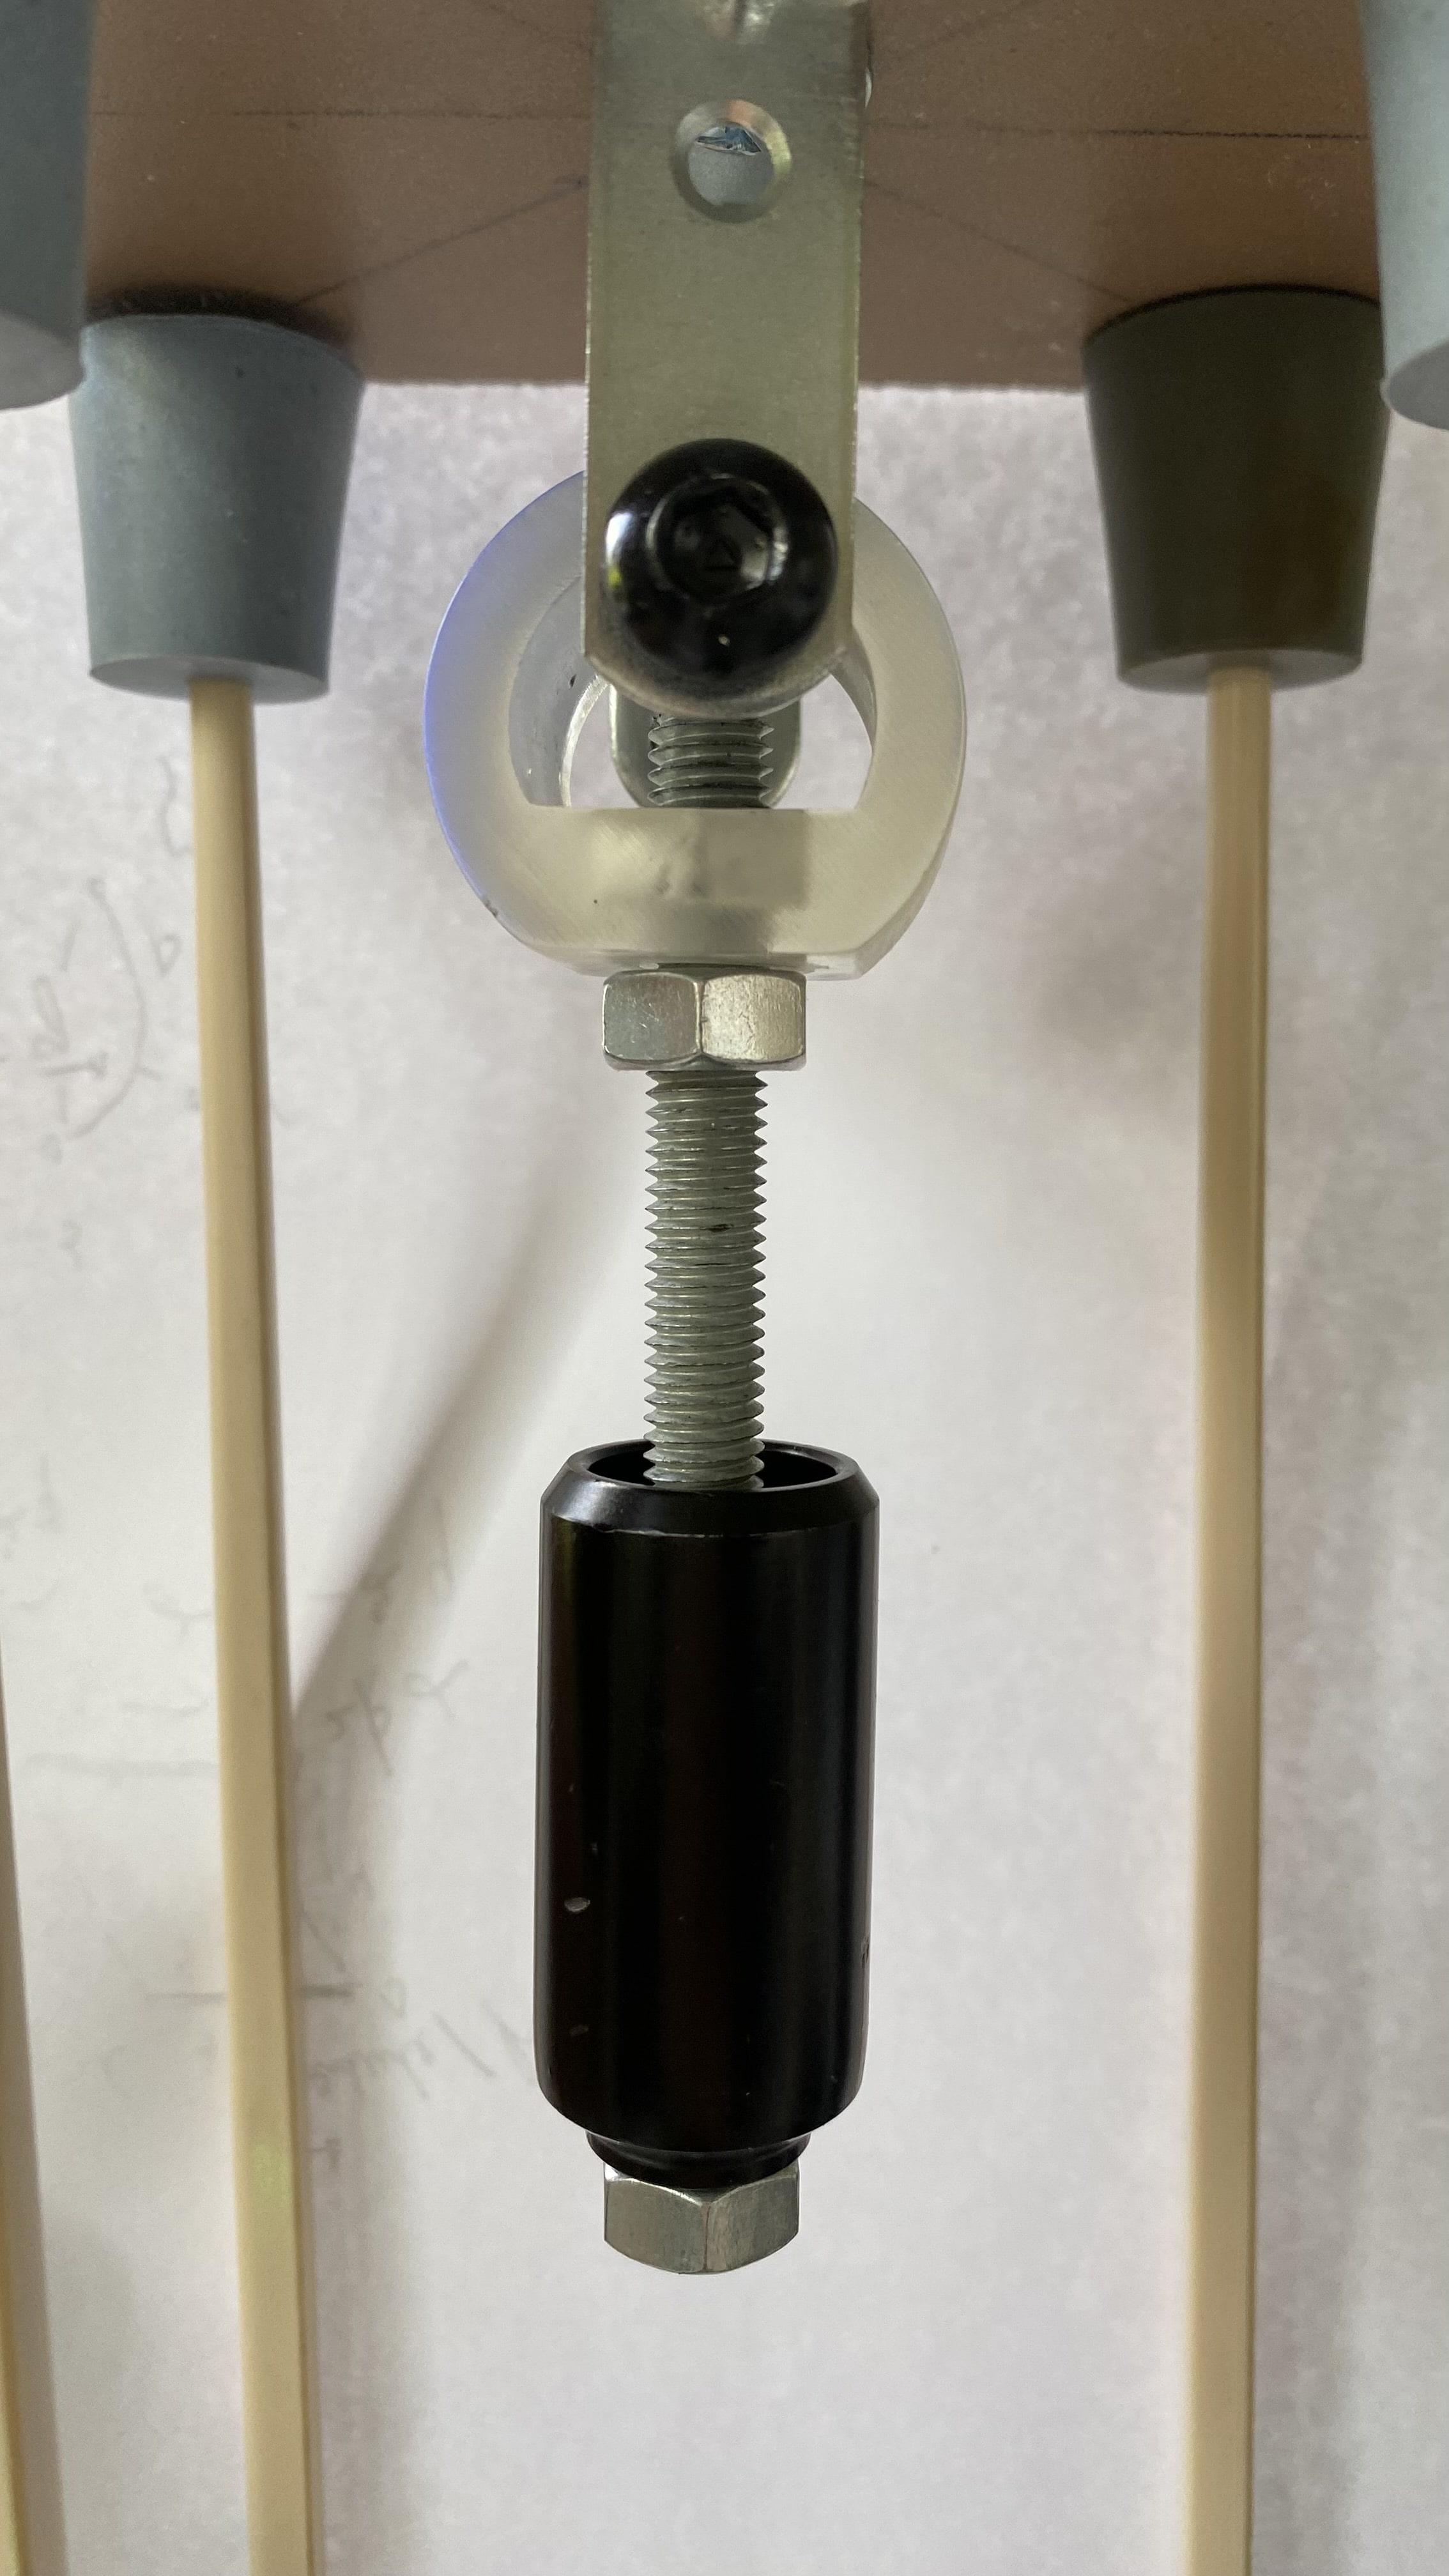
\includegraphics[width=0.6\textwidth]{C:/Users/noebo/OneDrive/Documents/Prépa/TIPE TMD/Présentation/Photos comp/IMG_E3392-min.JPG}
					\caption{Pendule}
				\end{figure}
			\end{column}
		\end{columns}
	\end{frame}

\begin{frame}{Construction de la maquette}
		\frametitle{Outil de mise en vibration}
		\begin{columns}
			\begin{column}{0.5\textwidth}
				\begin{figure}
					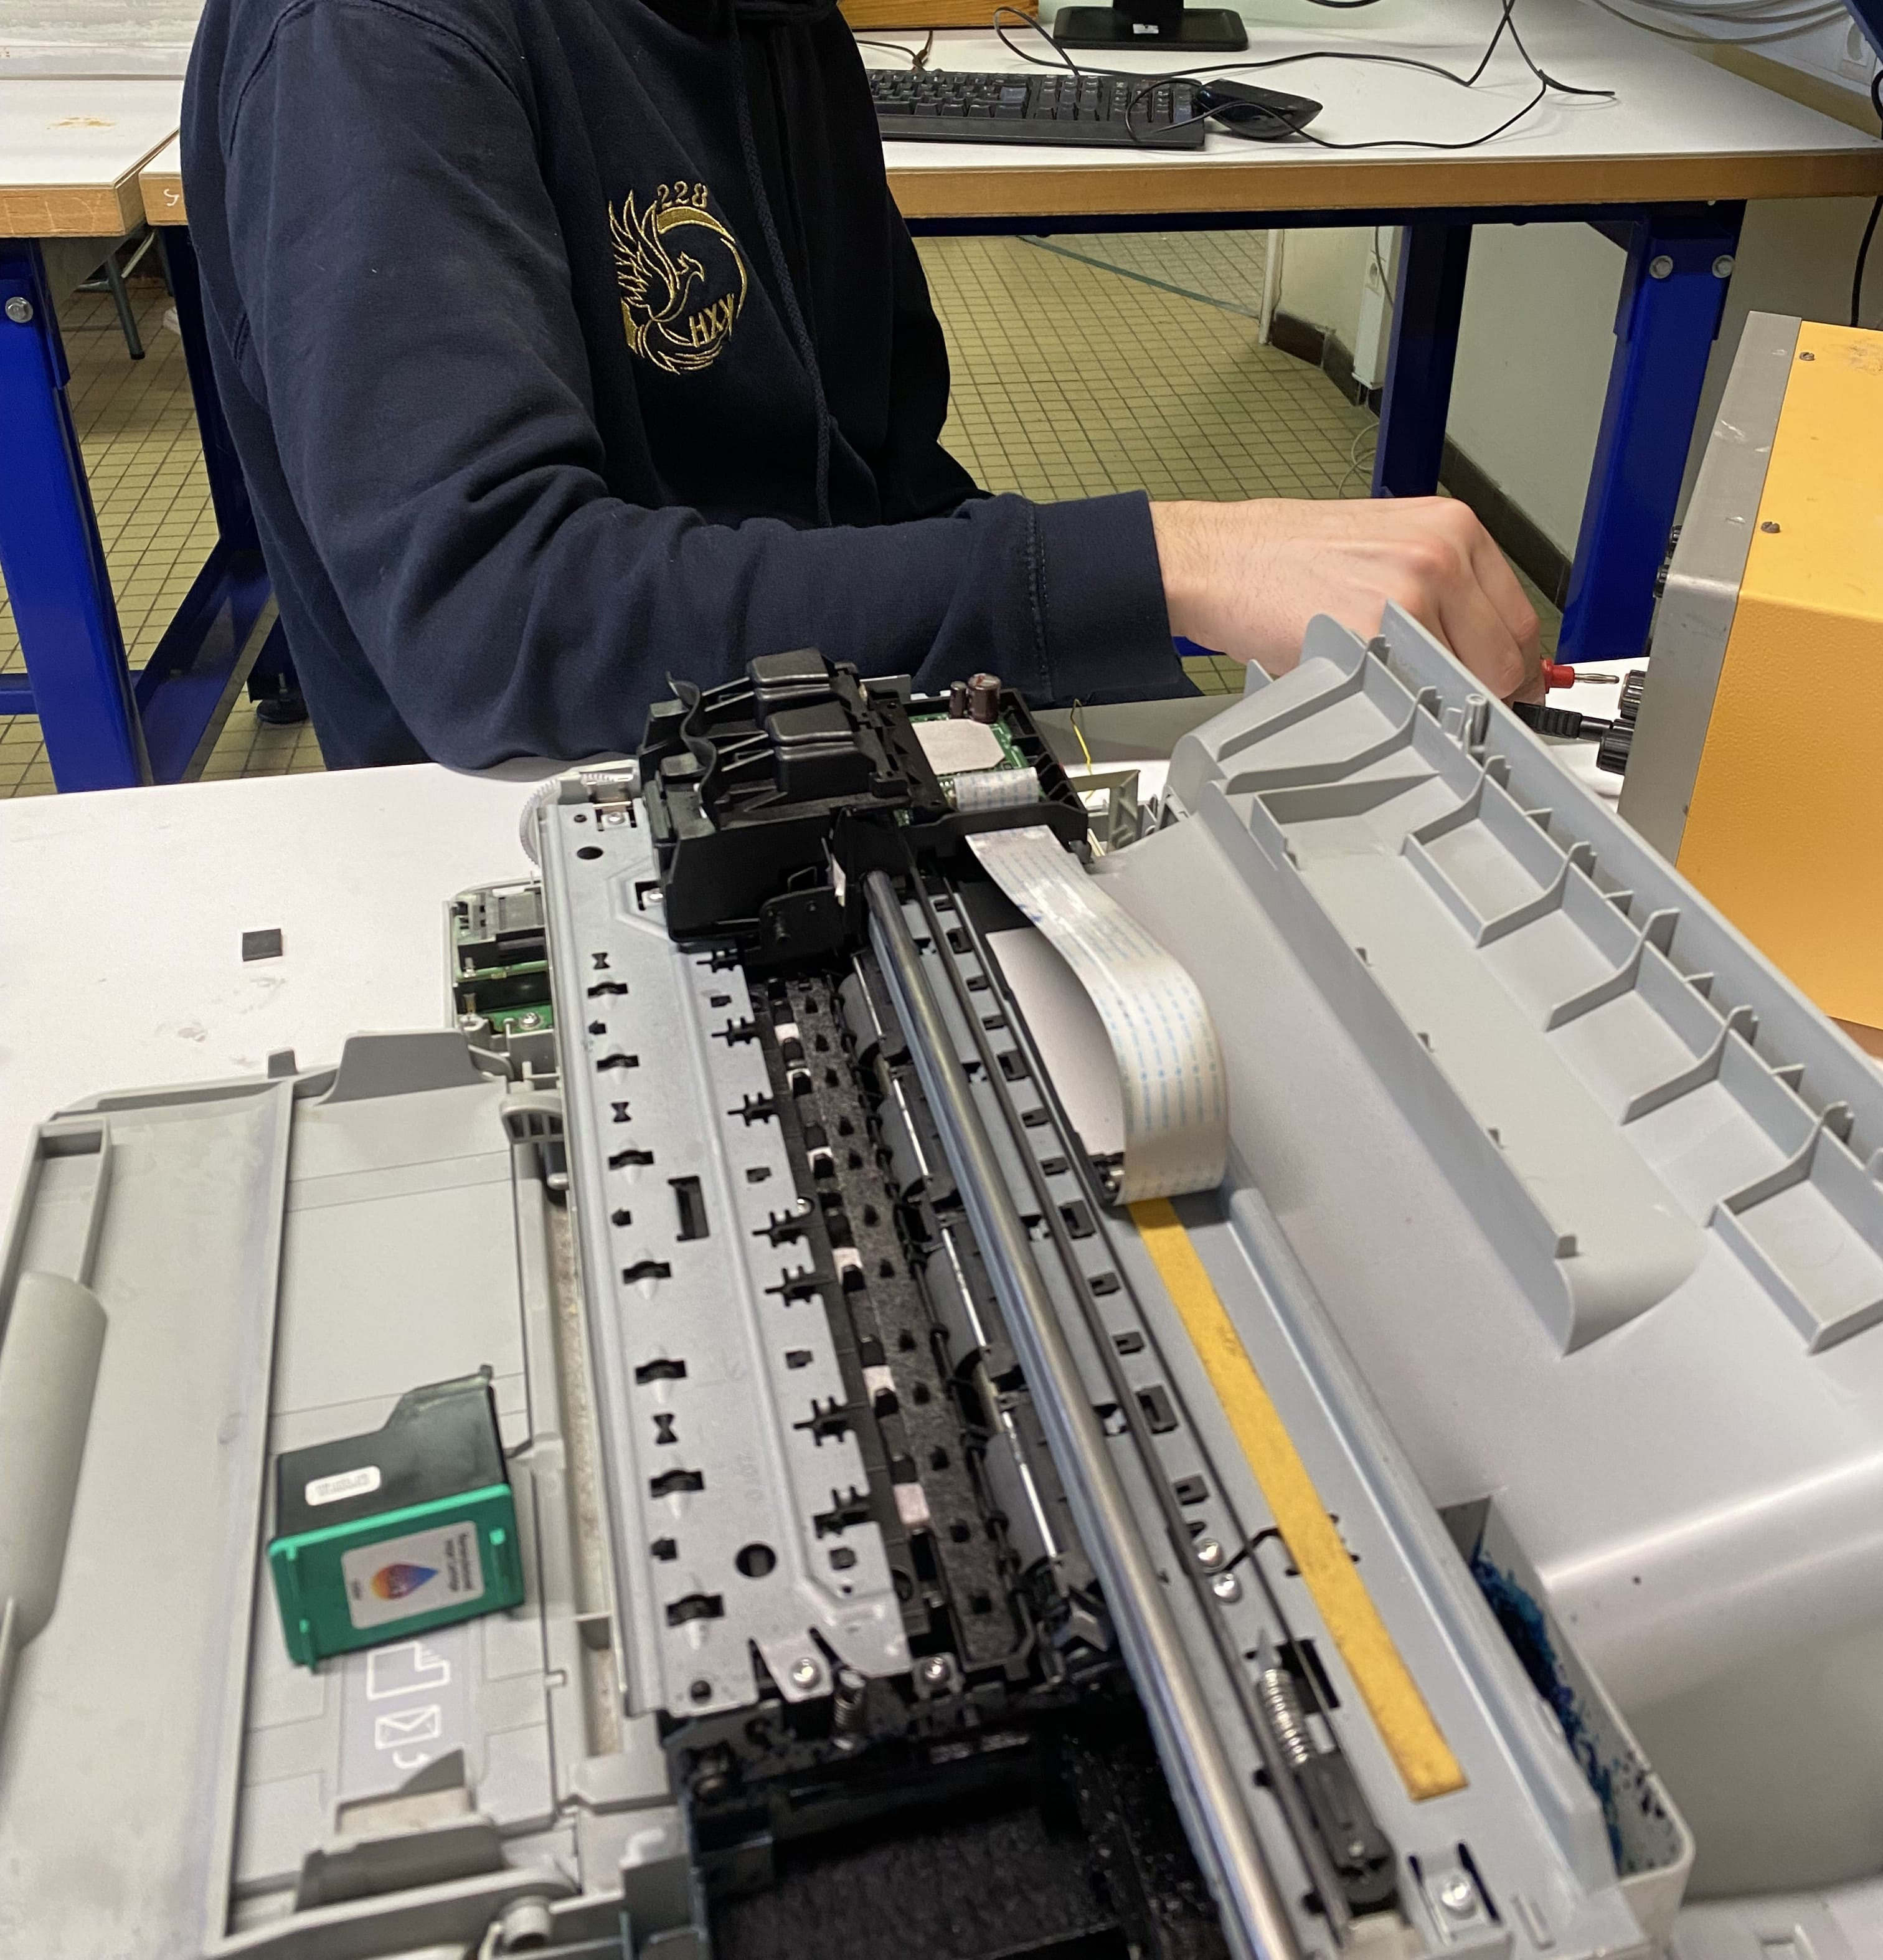
\includegraphics[width=0.8\textwidth]{C:/Users/noebo/OneDrive/Documents/Prépa/TIPE TMD/Présentation/Photos comp/IMG_2609-min.JPG}
					\caption{Guidage en translation d'une imprimante}
				\end{figure}
			\end{column}
			\begin{column}{0.5\textwidth}
				Inconvénients:
				\begin{itemize}
					\item Difficultés pour fixer la structure
					\item Fréquence non réglable \\
					\item Masse de la structure qui influe sur la vitesse
				\end{itemize}

			\end{column}
		\end{columns}
	\end{frame}

	
	\begin{frame}{Construction de la maquette}
		\frametitle{Outil de mise en vibration}
 
		\begin{columns}
			\begin{column}{0.5\textwidth}
				\begin{figure}
					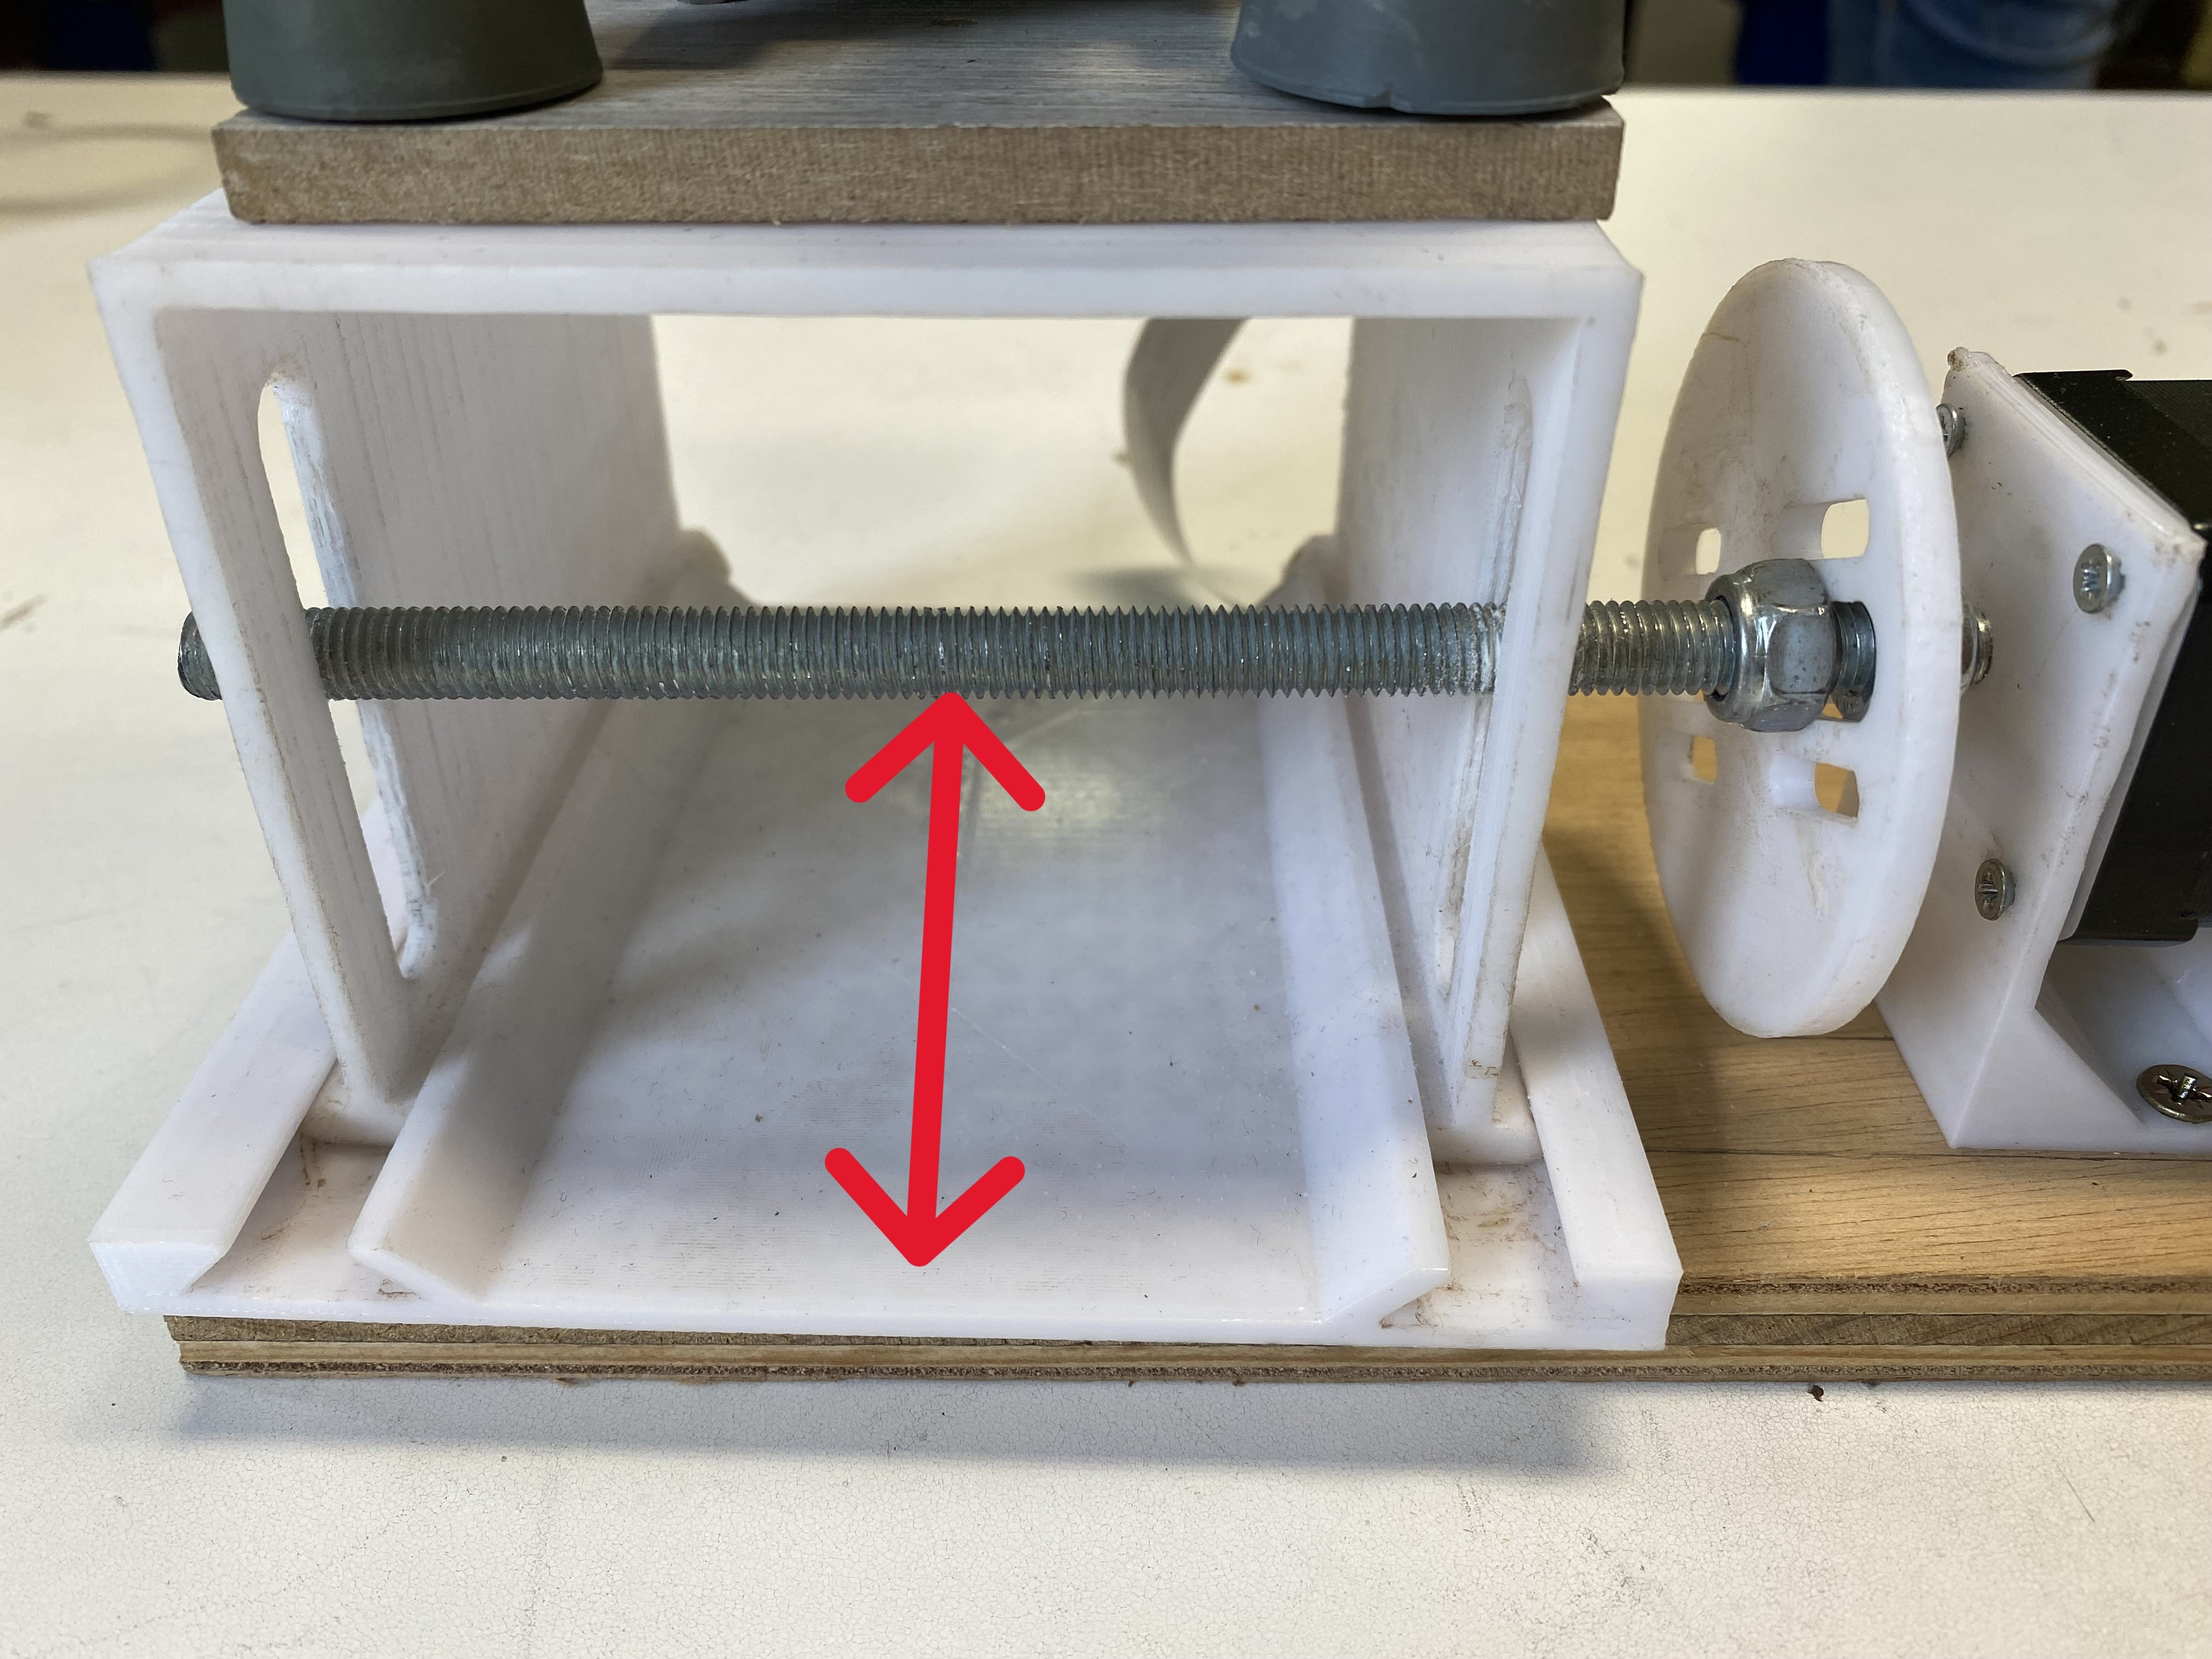
\includegraphics[width=\textwidth]{C:/Users/noebo/OneDrive/Documents/Prépa/TIPE TMD/Présentation/Photos comp/IMG_3367b-min.JPG}
					\caption{Mécanisme}
				\end{figure}
			\end{column}
			\begin{column}{0.5\textwidth}
				Avantages:
				\begin{itemize}
					\item\ Facilité pour fixer la structure
					\item Fréquence réglable \\
					\item Amplitude réglable 
				\end{itemize}
				\vspace{12pt}
				Inconvénients:
				
				\begin{itemize}
					\item Hystérésis
				\end{itemize}
			\end{column}
		\end{columns}
	\end{frame}

\begin{frame}{Outil de mise en vibration}
	\begin{figure}
		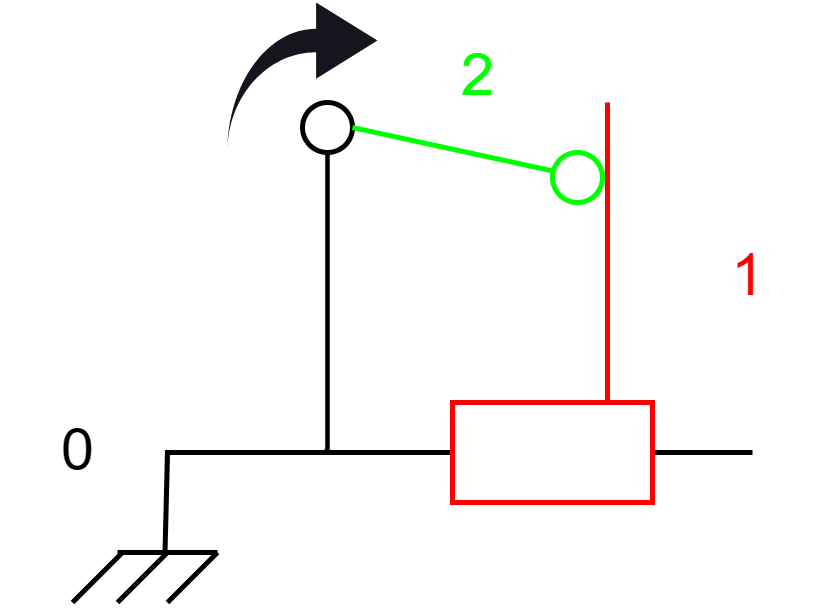
\includegraphics[width=0.5\textwidth]{C:/Users/noebo/OneDrive/Documents/Prépa/TIPE TMD/Présentation/Photos comp/Schema_oscillateur_position_droite.drawio-min.png}
		\caption{Schéma cinématique de l'outil de vibration}
	\end{figure}
\end{frame}

	\begin{frame}{Mise en vibration de la maquette}
	
	%schéma de la maquette avec des 2 accéléromètres
	\frametitle{Capteurs}
	\begin{columns}
		\begin{column}{0.25\textwidth}
			\begin{figure}
				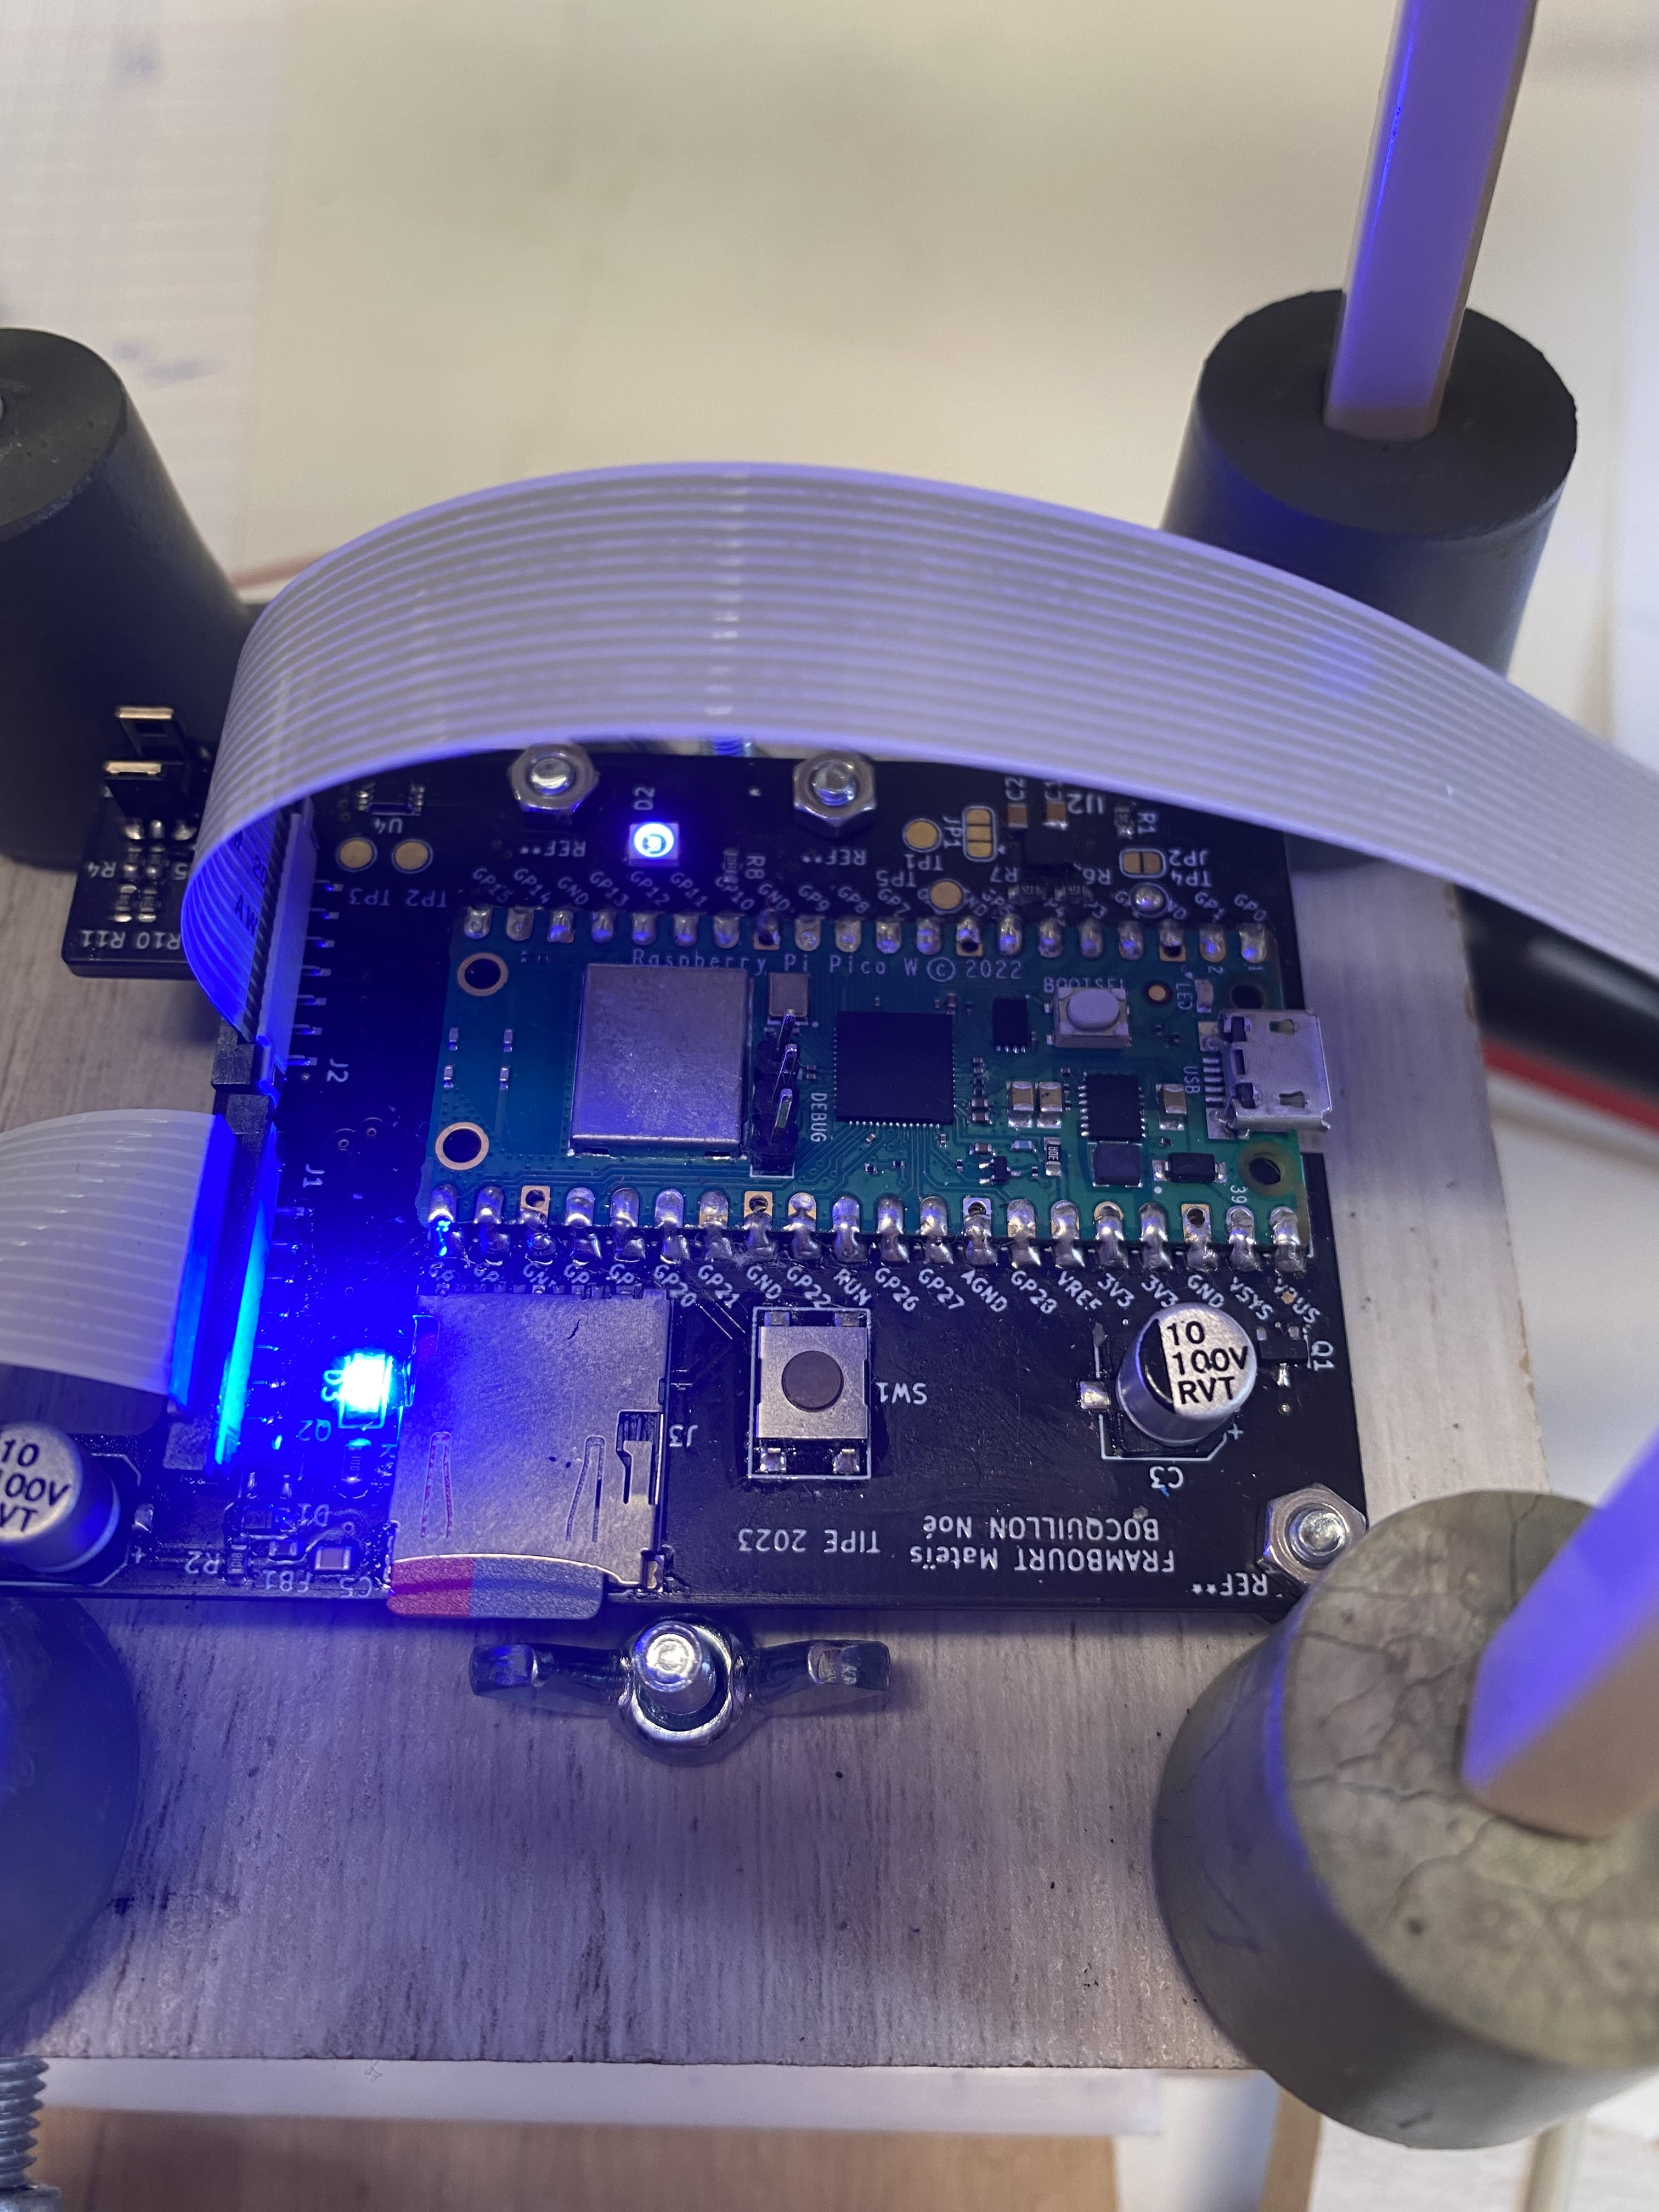
\includegraphics[width=\textwidth]{C:/Users/noebo/OneDrive/Documents/Prépa/TIPE TMD/Présentation/Photos comp/IMG_3378-min.JPG}
				\caption{Accéléromètre sur le socle}
			\end{figure}
		\end{column}
		\begin{column}{0.5\textwidth}
			\begin{figure}
				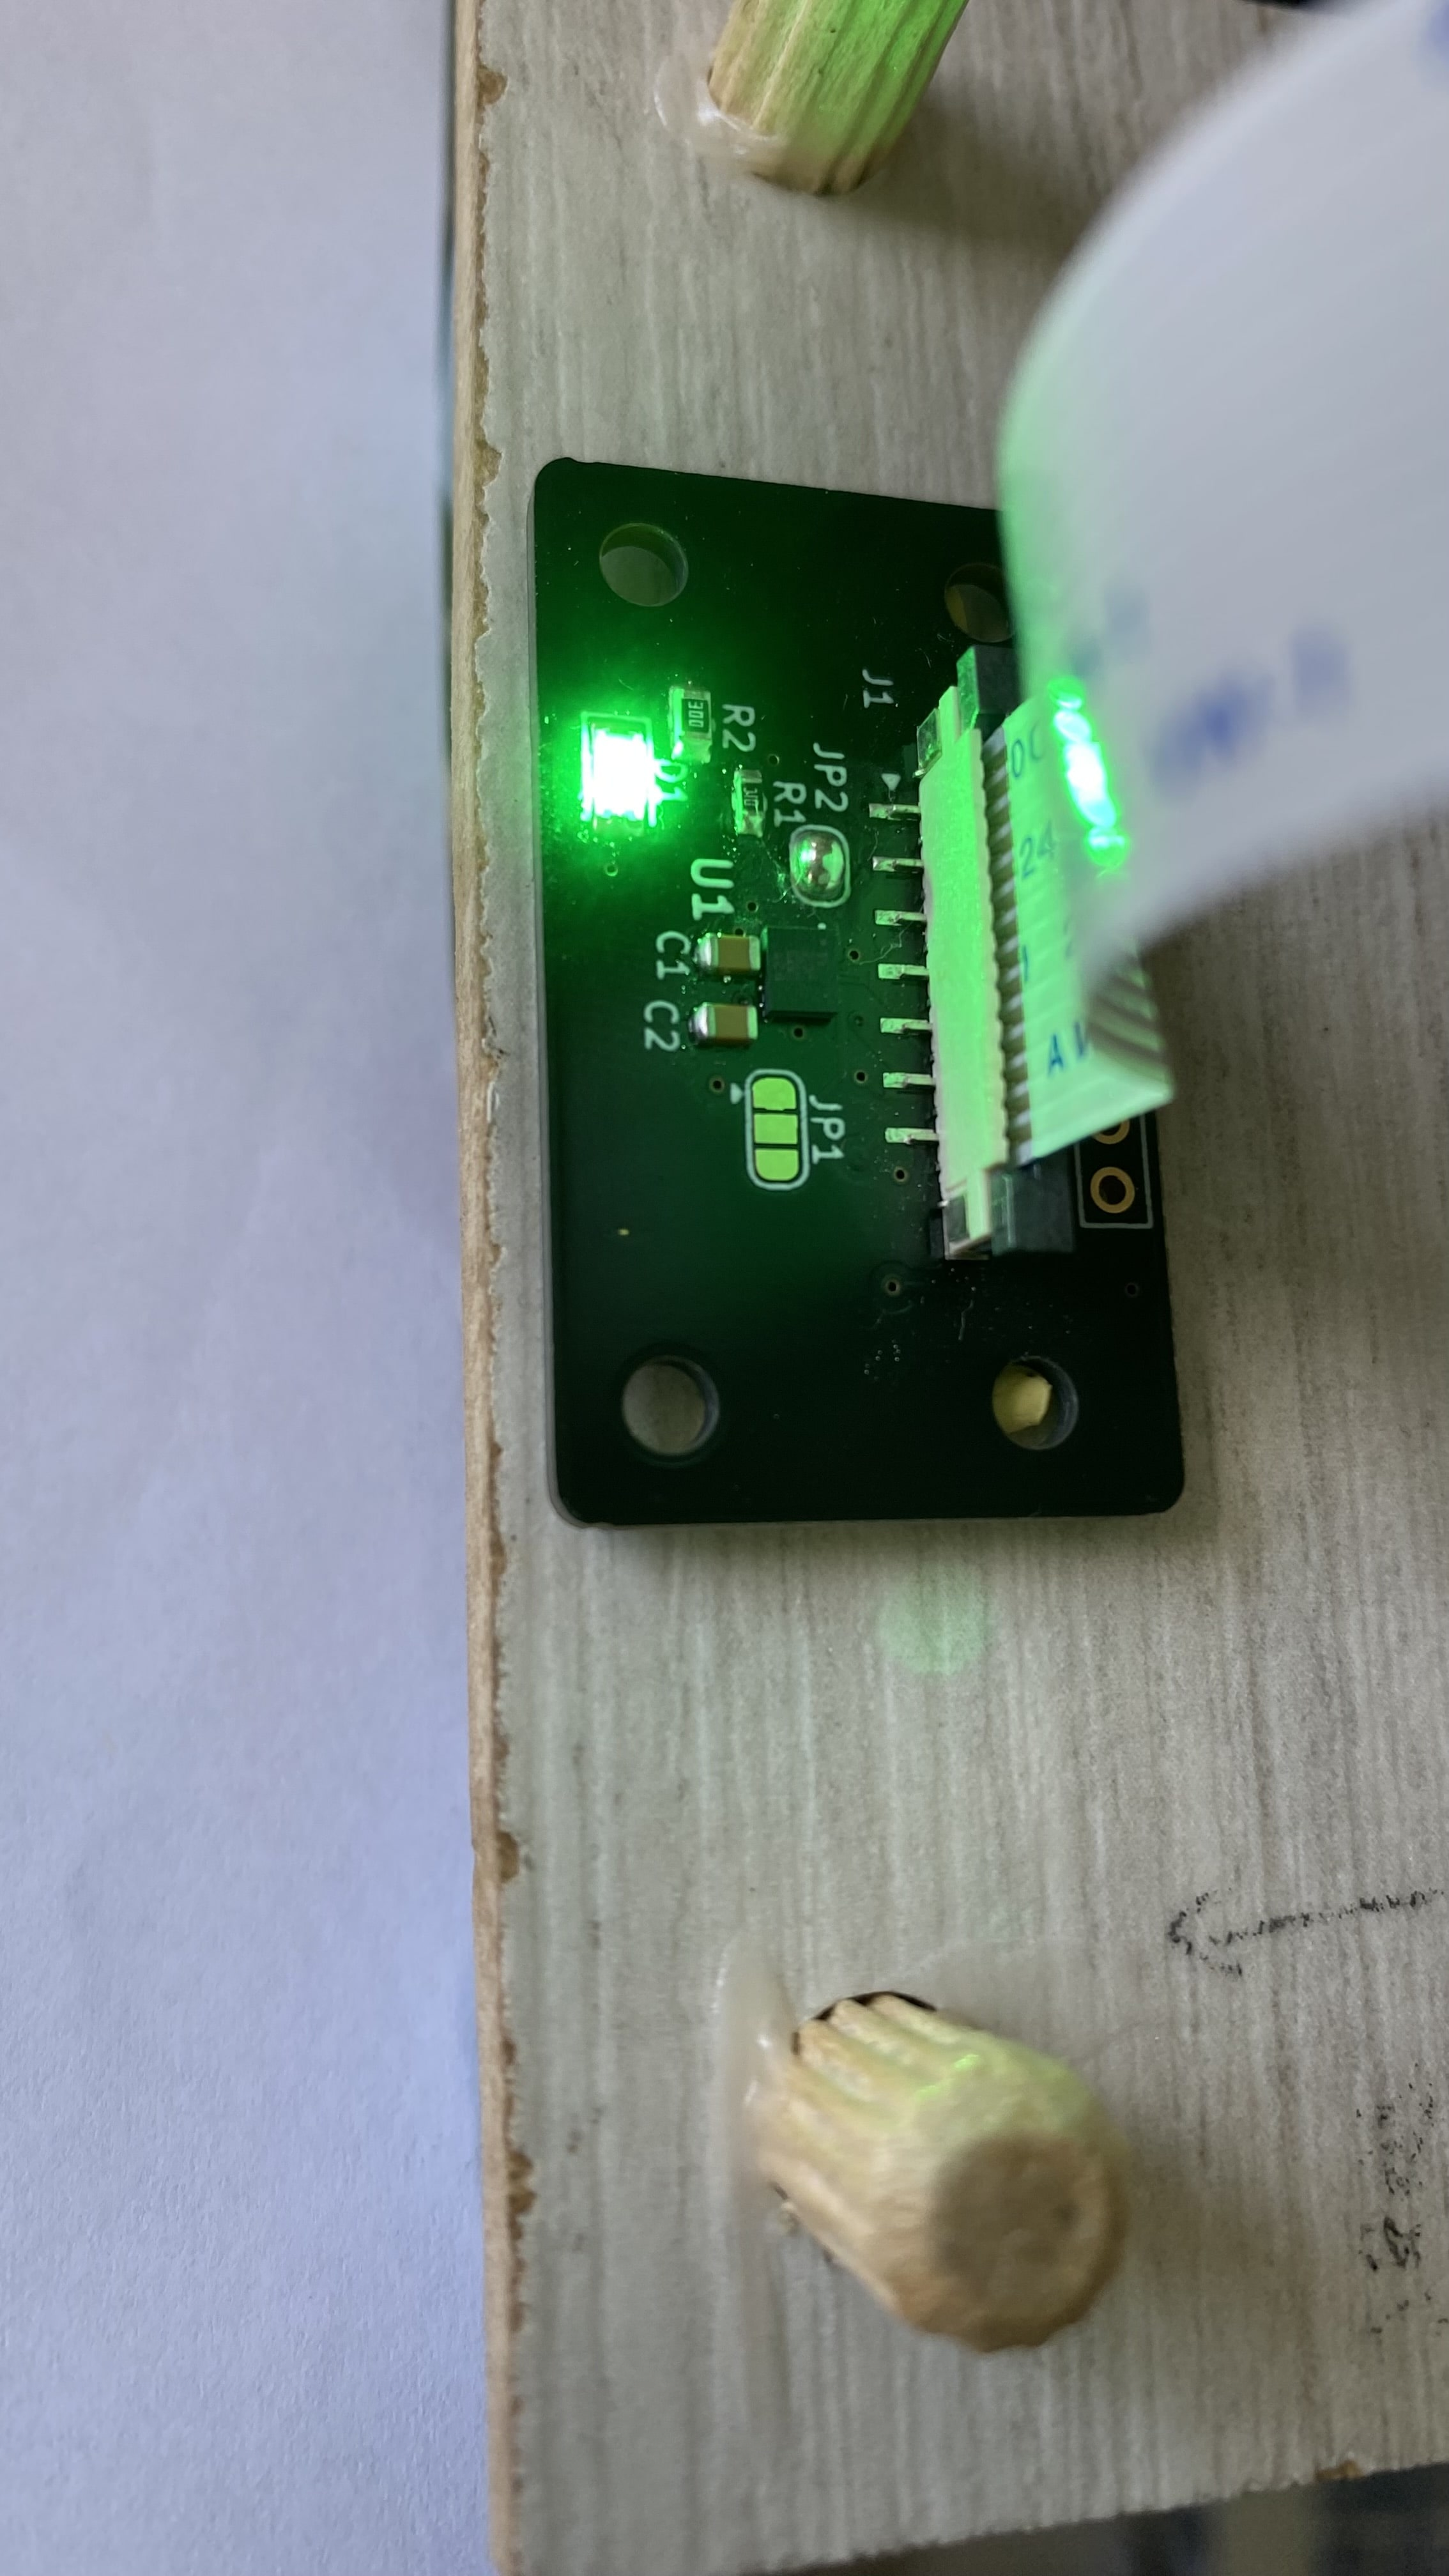
\includegraphics[width=0.5\textwidth]{C:/Users/noebo/OneDrive/Documents/Prépa/TIPE TMD/Présentation/Photos comp/IMG_E3393-min.JPG}
				\caption{Accéléromètre du haut}
			\end{figure}
		\end{column}
	\end{columns}
	Permet de tracer des diagrammes de Bode 
\end{frame}
	
\section{Théorie}

\begin{frame}{Détermination du modèle théorique}
 Modélisation de la maquette sans pendule:\vspace{12 pt}
	\begin{columns}
		\begin{column}{0.5\textwidth}
			\begin{figure}
				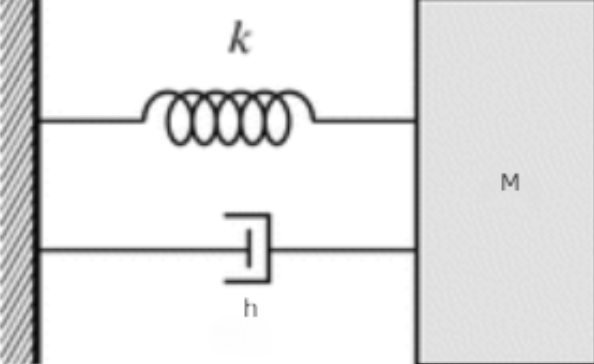
\includegraphics[width=0.6\textwidth]{C:/Users/noebo/OneDrive/Documents/Prépa/TIPE TMD/Présentation/Modélisation sans pendule.PNG}
				\caption{Modélisation sans pendule}
			\end{figure}
		\end{column}
		\begin{column}{0.6\textwidth}
			PFD à la tour:
			\begin{equation*}
				M\ddot{x} = -kx -h\dot{x} + f(t)
			\end{equation*}
			Ce qui donne la fonction de transfert : 
			$H(\omega)=\frac{X}{F}=\frac{1}{1+j*\frac{h}{k}*\omega-\frac{M}{k}*\omega^{2}}$
		\end{column}
	\end{columns}
\end{frame}	



	
\begin{frame}
	Cette première expérience permet de déterminer les valeurs de k et h 
\end{frame}


\begin{frame}{Élaboration d'un modèle théorique}
	\frametitle{Modélisation du système avec pendule}
	Oscillations linéaires , on peut modéliser le pendule par un système masse ressort
	\begin{columns}
		\begin{column}{0.5\textwidth}
			\begin{figure}
				\centering
				\includegraphics[width=1\textwidth]{"C:/Users/noebo/OneDrive/Documents/Prépa/TIPE TMD/Présentation/ModelisationMP-min.png"}
				\caption{Modèle équivalent du système}
			\end{figure}
		\end{column}
		\begin{column}{0.5\textwidth}
			\begin{itemize}
				\item m=Masse du pendule
				\item M=Masse de la tour
				\item $k_{1}$=Coefficient de raideur élastique du pendule
				\item k=Coefficient de raideur élastique (Baguettes + bouchons dans notre modèle)
				\item $h_{1}$= coefficient de frottement du pendule 
				\item h=coefficient de frottement de la tour
			\end{itemize}	
		\end{column}
	\end{columns}
	
\end{frame}

%\begin{frame}{Modélisation du système avec pendule}
	%PFD à la tour sans pendule ni excitation extérieure (Correspond au Dirac): 
%	\begin{equation}\label{key}
	%	\ddot{x} + \frac{h}{M}\dot{x}  + \frac{K}{M}x = 0
%	\end{equation}\vspace{24pt}
%	Période naturelle de la tour:$ T = 2\pi\frac{1}{\sqrt{\frac{K}{M}-\frac{h}{4M^2}}}$\\
%	\vspace{12 pt}
%	Mesure de T et de h expérimentalement :\\ Obtention de la valeur de K
%\end{frame}

\begin{frame}{Élaboration d'un modèle théorique}
	\frametitle{Équations du système}	
	L'excitation extérieure est modélisée par une force $f_{0}(t)$ appliquée à la tour\vspace{12pt}
	PFD à ${tour + TMD}$:
	\begin{equation}\label{key}
		M\ddot{x} + m(\ddot{x}+\ddot{u}) +h\dot{x} + kx = f_{0}(t)
	\end{equation}\\
	\vspace{12pt}
	PFD  au TMD uniquement:
	\begin{equation}
		m(\ddot{x}+\ddot{u}) + h_{1}\dot{u} + k_{1}u = 0
	\end{equation}\\

	
\end{frame}

\begin{frame}{Fonctions de transfert du système}
	
\begin{empheq}[left=\empheqlbrace]{align*}
	H1(\omega)&=\frac{U}{X}= \frac{m\omega^{2}}{k_{1}+jh_{1}\omega-m\omega^{2}}\\
	H2(\omega)&=\frac{X}{\frac{F_{0}}{k}}= \frac{1}{1+j\frac{h}{k}\omega-\frac{(M+m)}{k}\omega^2-\frac{H1(\omega)}{k}\omega^2}
\end{empheq}
\vspace{12 pt}

H2 représente le rapport de l'amplitude de l'accélération ressentie par les occupants de  la tour et de l'amplitude de l'accélération extérieure que subit la tour


	
	
\end{frame}
\section{Mise en vibration de la maquette}



\begin{frame}{Mise en vibration de la maquette}
	\frametitle{Première expérience:Réponse à une excitation sinusoïdale}
	\begin{columns}
		\begin{column}{0.35\textwidth}
			\alert{Simulation d'un séisme}
		\end{column}
		\begin{column}{0.7\textwidth}
			Conditions de l'expérience :
			\begin{itemize}
				\item Excentration la plus faible 
				\item Oscillations dans un seul plan
				\item Plage de fréquences :[0.5 hz;3.5 hz]
			\end{itemize}	
		\end{column}
	\end{columns}
	
	
	\begin{figure}
		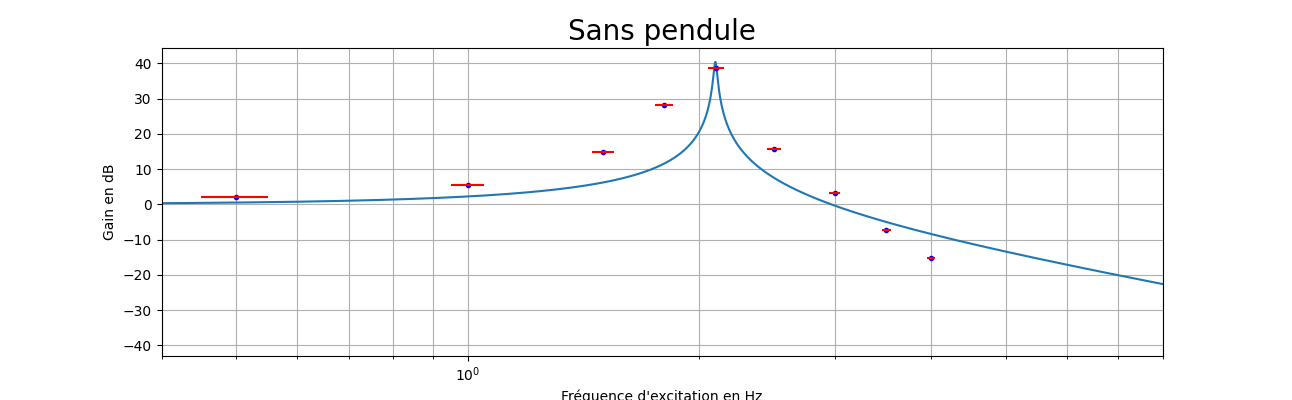
\includegraphics[scale=0.36]{"C:/Users/noebo/OneDrive/Documents/Prépa/TIPE TMD/Présentation/Données pi avec comparaison/Sans pendule.png"}
		
	\end{figure}
Cette première expérience sans pendule permet de trouver les valeurs de k et de h de notre système 
k=2,5
h=0,005
\end{frame}

	
	\begin{frame}{Première expérience:Réponse à une excitation sinusoïdale}
	Changement de la longueur du pendule:

		
		\begin{figure}
		\centering
		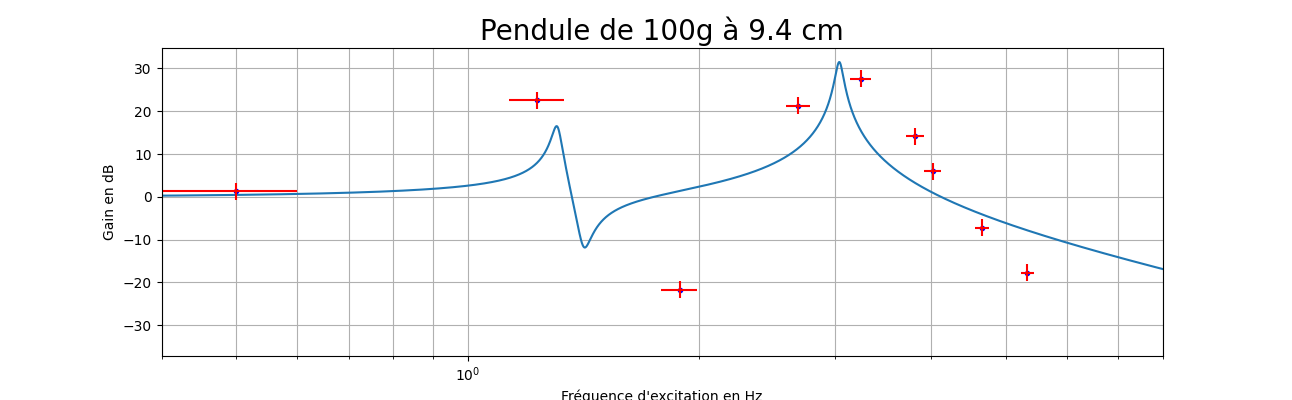
\includegraphics[scale=0.33]{C:/Users/noebo/OneDrive/Documents/Prépa/TIPE TMD/Présentation/Données pi avec comparaison/Pendule 100g à 9,4 cm.png}
		
		
		\centering
		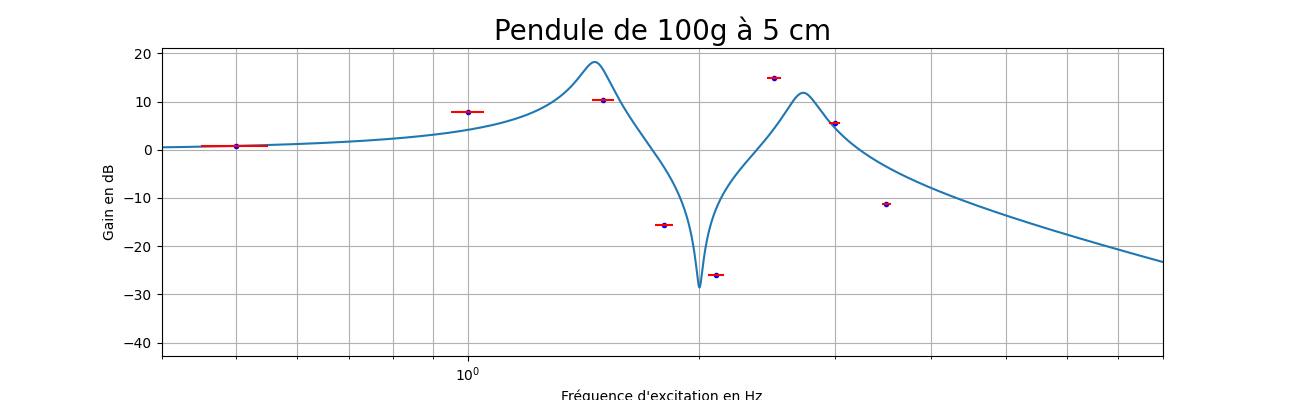
\includegraphics[scale=0.33]{C:/Users/noebo/OneDrive/Documents/Prépa/TIPE TMD/Présentation/Données pi avec comparaison/Pendule 100g à 5 cm.png}
		\end{figure}
	\end{frame}
	
	\begin{frame}{Mise en vibration de la maquette}
		\frametitle{Première expérience:Réponse à une excitation sinusoïdale}
		\centering
		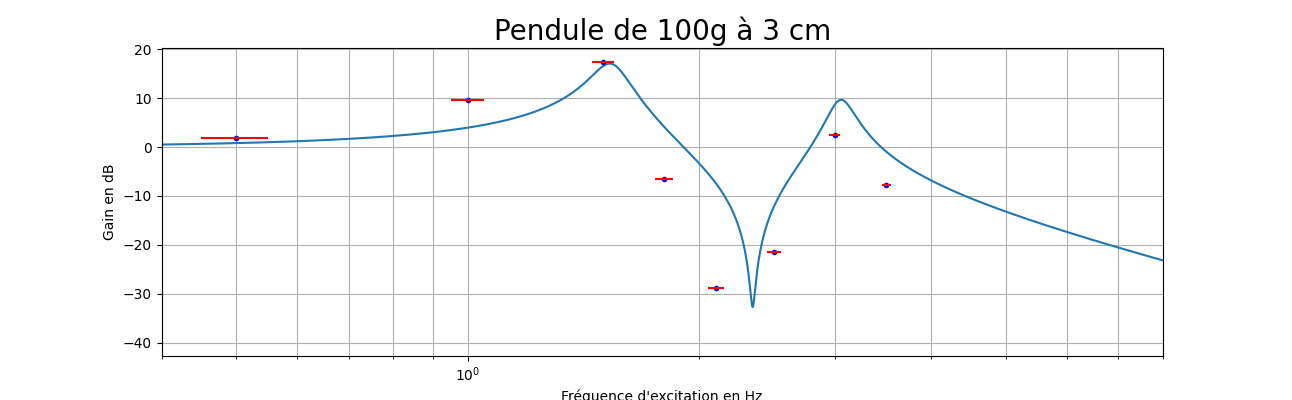
\includegraphics[scale=0.33]{C:/Users/noebo/OneDrive/Documents/Prépa/TIPE TMD/Présentation/Données pi avec comparaison/Pendule 100g à 3 cm.png}
		\\
		\vspace{12pt}
		Observations:
		\begin{itemize}
			\item Réduction de l'amplitude des oscillations
			\item Influence du centre de gravité du pendule
			\item Décalage de la fréquence de résonance  
		\end{itemize}
		
	\end{frame}


	
	\begin{frame}{Mise en vibration de la maquette}
		\frametitle{Première expérience:Réponse à une excitation sinusoïdale}	
		Changement de la masse du pendule:
		\centering
		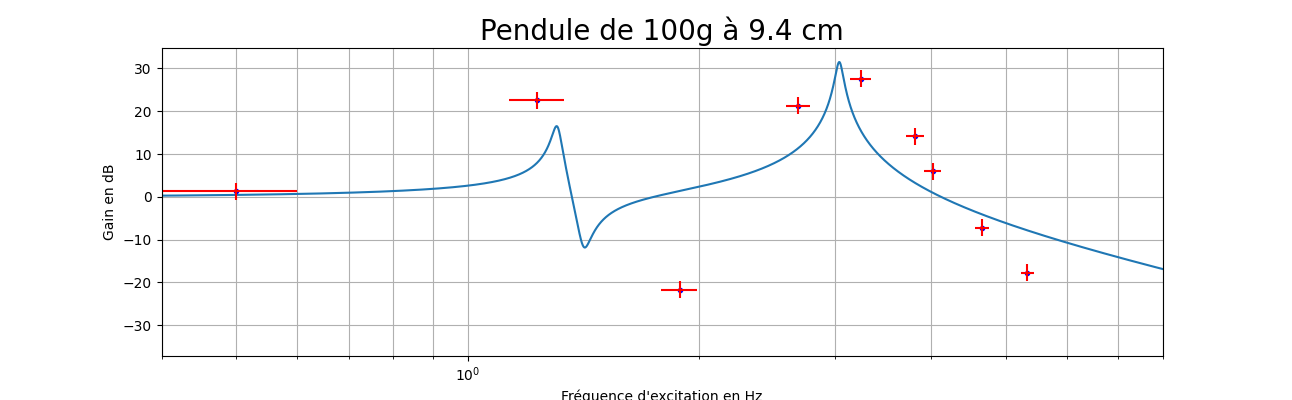
\includegraphics[scale=0.33]{C:/Users/noebo/OneDrive/Documents/Prépa/TIPE TMD/Présentation/Données pi avec comparaison/Pendule 100g à 9,4 cm.png}
		
		
		\centering
		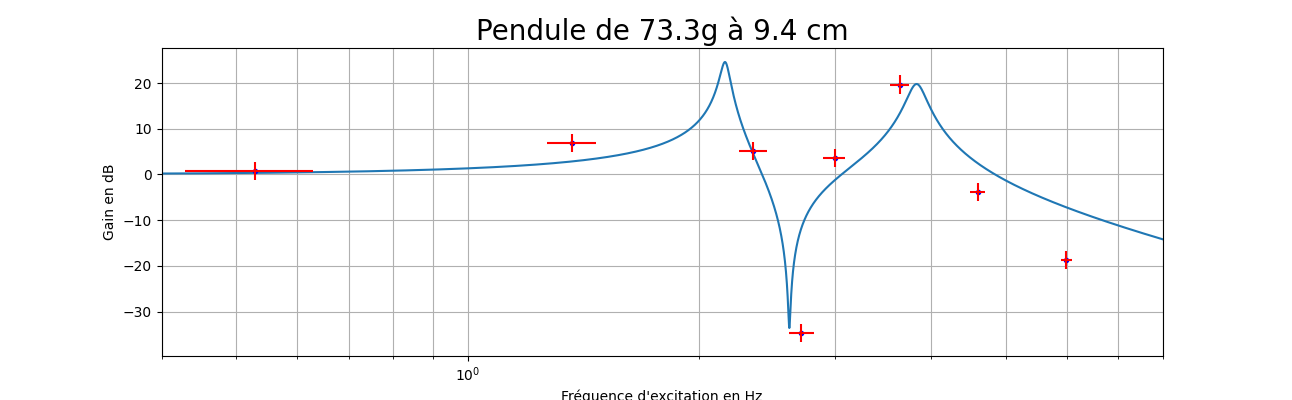
\includegraphics[scale=0.33]{C:/Users/noebo/OneDrive/Documents/Prépa/TIPE TMD/Présentation/Données pi avec comparaison/Pendule 73.3g à 9,4 cm.png}
		
		
	\end{frame}
	
	
	
	
	\begin{frame}{Mise en vibration de la maquette}
		\frametitle{Deuxième expérience:Réponse à une excitation brève}
		\begin{columns}
			\begin{column}{0.5\textwidth}
				\alert{Simulation d'une rafale de vent}
				\begin{figure}
					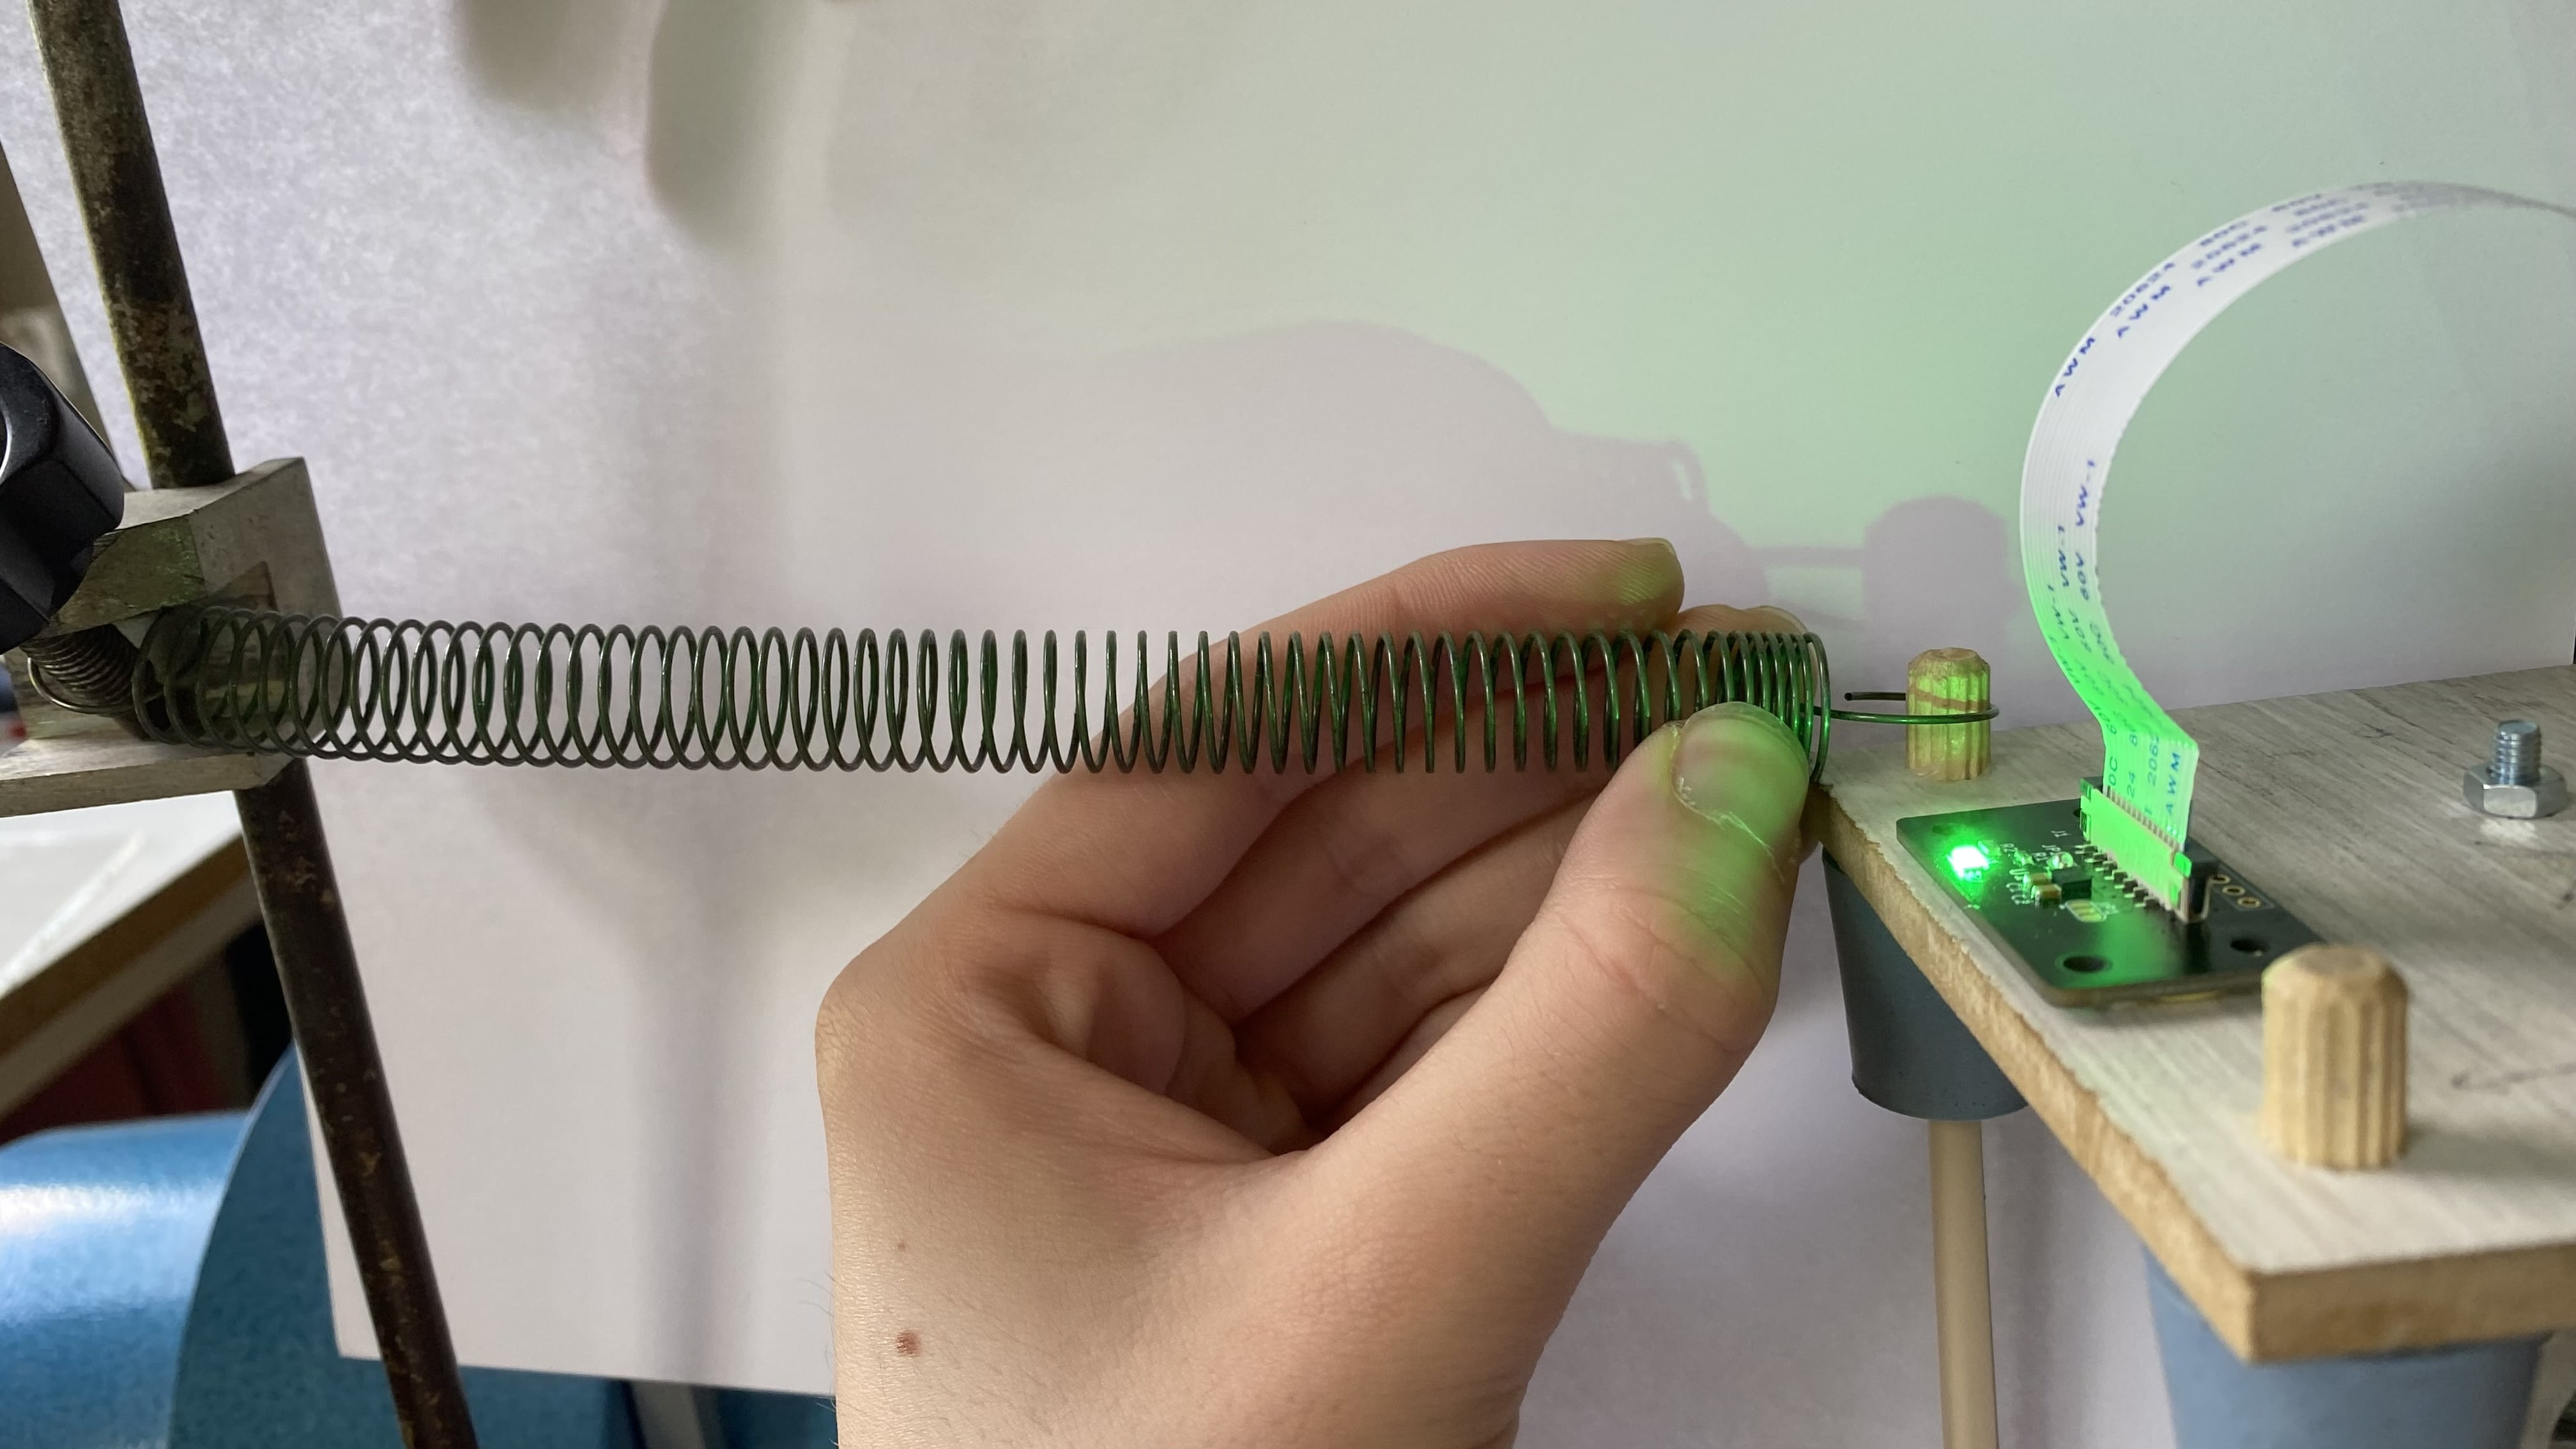
\includegraphics[width=\textwidth]{C:/Users/noebo/OneDrive/Documents/Prépa/TIPE TMD/Présentation/Photos comp/IMG_E3390-min.JPG}
					\caption{Excitation brève}
				\end{figure}
			\end{column}
			\begin{column}{0.5\textwidth}
				Conditions de l'expérience :
				\begin{itemize}
					\item Dirac avec un ressort 
					\item Oscillations dans un seul plan
				\end{itemize}	
			\end{column}
		\end{columns}
	\end{frame}
	
	
	
	
	\begin{frame}{Mise en vibration de la maquette}
		\frametitle{Deuxième expérience:Réponse à une excitation brève}
		\vspace{12pt}
		\begin{figure}
				\includegraphics[width=0.85\textwidth]{C:/Users/noebo/OneDrive/Documents/Prépa/TIPE TMD/Présentation/Photos comp/coup de vent comparaison-min.png}
				\caption{Réponse temporelle à une excitation brève}
				\tiny{\small{\textcolor{orange}{Avec pendule de 100g à 9,4 cm}\\
				\textcolor{blue}{Sans pendule}}}
			
			
	\end{figure}
	\end{frame}





	
	%\begin{frame}{explications}
	%dissipation d'énergie dans le pendule , opposition de phases , rapport des pulsations naturelles
	%\end{frame}
	
	%\begin{frame}{limites}
	%	dimension peu adaptées (rapport de la taille et de la masse du pendule par rapport à la structure\\structure trop élastique qui entraine parfois des non linéarité à la fréquence de résonance )
	%\end{frame}
	
	%\begin{frame}{ce qu'on aurait aimé faire}
	%comparaison avec un modèle informatique\\
	%	plus de variations de paramètres\\
	%	mettre le pendule dans un fluide pour plus de viscosité
	%\end{frame}
	
\section{Conclusion}
\begin{frame}{Conclusion}
	\begin{itemize}
		\item Rapport entre masse du pendule et de la structure peu assimilable au réel
		\item Élasticité de la maquette trop importante
	\end{itemize}
\end{frame}	
	
	
\section{Annexes}
	
	\begin{frame}
		\frametitle{Annexes}
		Graphique et explication des mesures des coefficients de raideur\\
		Dimension de la tour\\
		schéma solidworks outil de mise en vibration \\
		détermination des incertitudes\\
		équation et fonction de transfert\\
		
	\end{frame}

\begin{frame}{Dimension de la maquette}
			\begin{columns}
		\begin{column}{0.5\textwidth}
			\begin{figure}
				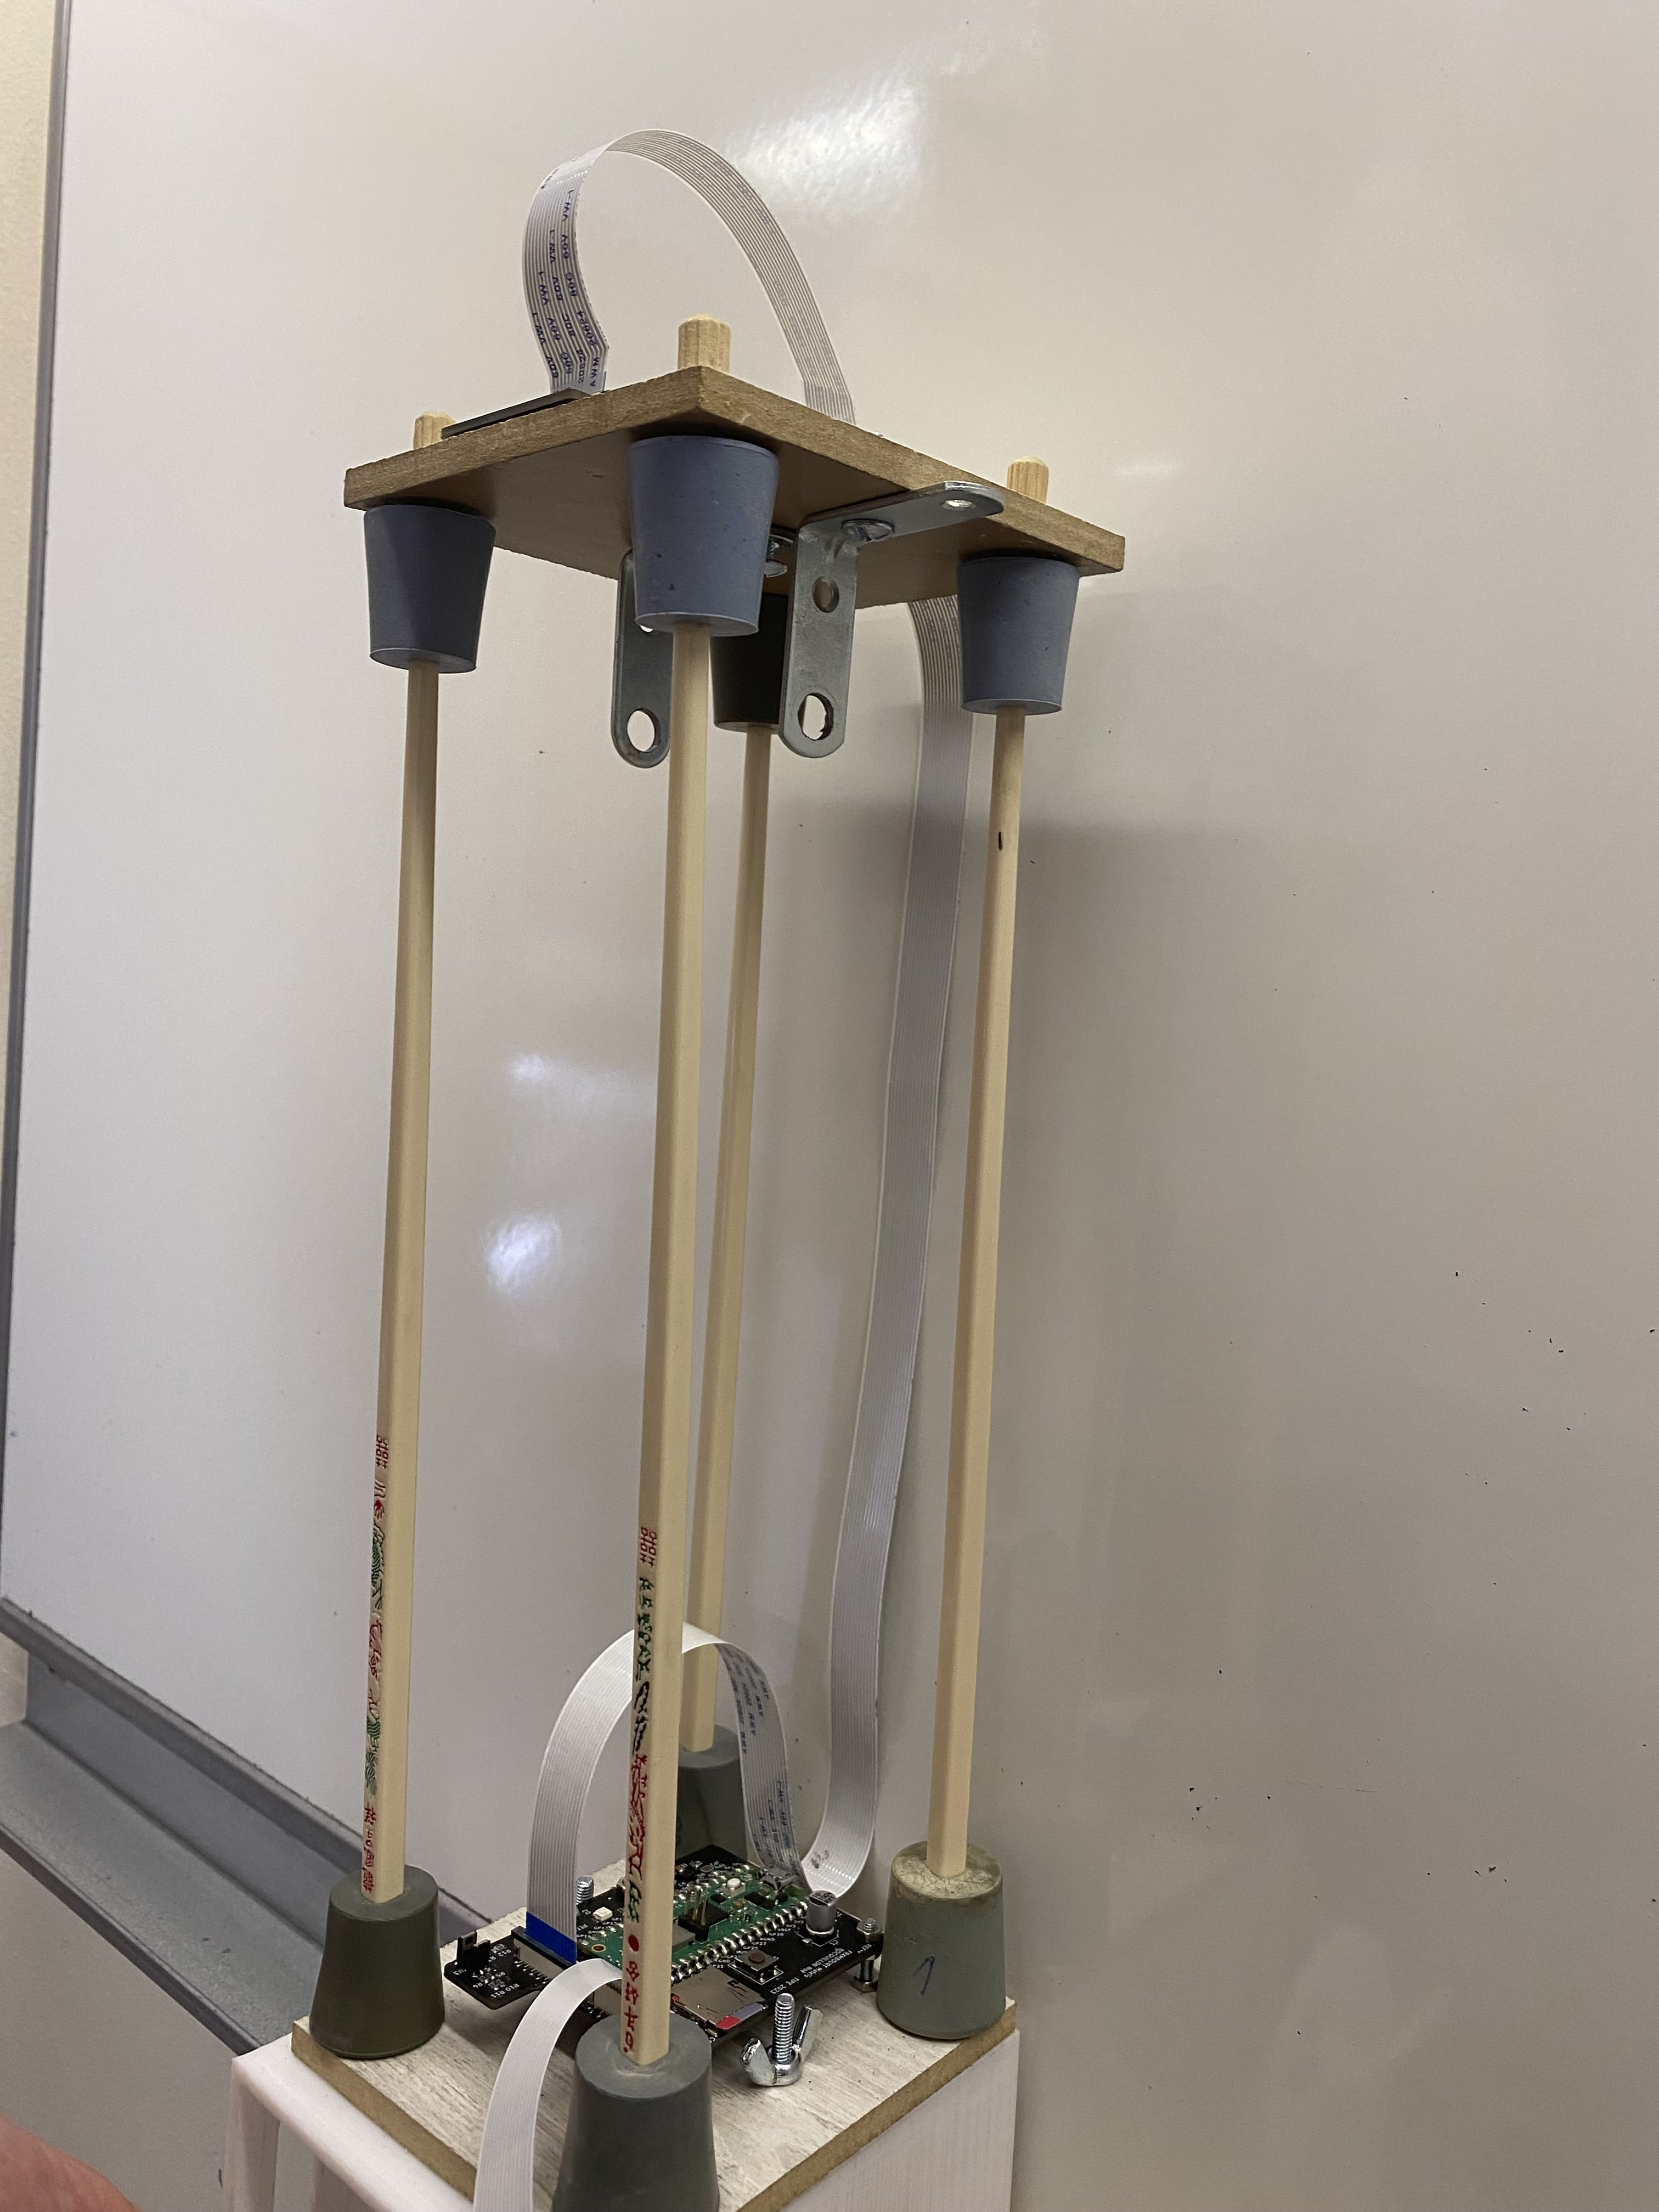
\includegraphics[width=0.8\textwidth]{C:/Users/noebo/OneDrive/Documents/Prépa/TIPE TMD/Présentation/Photos comp/IMG_3380-min.JPG}
				\caption{Maquette de l'immeuble}
			\end{figure}
		\end{column}
		\begin{column}{0.5\textwidth}
			\begin{itemize}
				\item  Hauteur : $31,4 cm \pm 0,2 cm$
				\item  Dimension du socle et du toit : $10 cm x 11 cm \pm 0,2 cm$
				\item Masse de la maquette (non équipée) :$ 315,8 g \pm 0,1g $
				\item Masse de la maquette (pendule sans masse): $410,7 g \pm 0,1 g$
				\item Longueur de la tige filetée : $10cm \pm 0,2cm$
				\item Masse de la tige filetée : $ 30,3 g \pm 0,1$
			\end{itemize}
			
		\end{column}
	\end{columns}
\end{frame}


\begin{frame}{Mesure du coefficient de raideur de la tour}
	%explications Mateis
				\begin{columns}
		\begin{column}{0.5\textwidth}
			\begin{figure}
				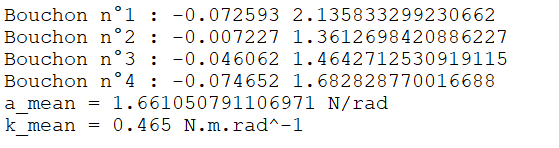
\includegraphics[width=0.7\textwidth]{C:/Users/noebo/OneDrive/Documents/Prépa/TIPE TMD/Présentation/Photos comp/valeur coef raideur-min.png}
				\caption{Détermination du coefficient de raideur élastique de la tour}
			\end{figure}
		\end{column}
		\begin{column}{0.5\textwidth}
				\begin{figure}
				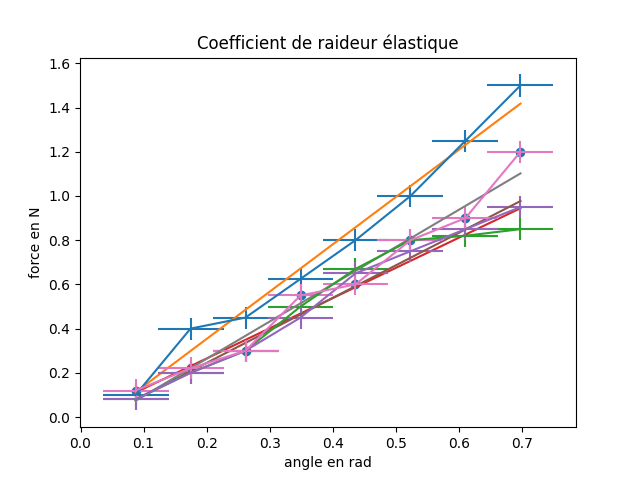
\includegraphics[width=0.7\textwidth]{C:/Users/noebo/OneDrive/Documents/Prépa/TIPE TMD/Présentation/Photos comp/coef raideur-min.png}
				\caption{Résultats python}
			\end{figure}
		\end{column}
	\end{columns}
  $K=3,72 N.m.rad^{-1}\pm ?$
  
  
  Incertitudes: Dynamomètre: 0,05 N \\
  Mesure des angles : 3 degrés 
\end{frame}

\begin{frame}{Outil de mise en vibration}

	\begin{columns}
		\begin{column}{0.5\textwidth}
			\begin{figure}
				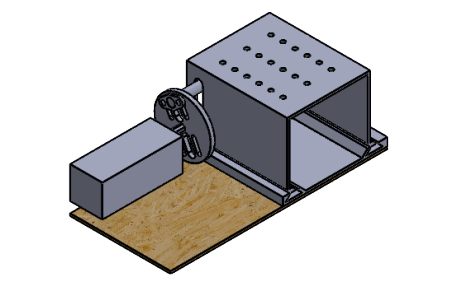
\includegraphics[width=0.8\textwidth]{C:/Users/noebo/OneDrive/Documents/Prépa/TIPE TMD/Présentation/Photos comp/schéma axe lineaire-min.png}
				\caption{Schéma de l'outil de mise en vibration}
			\end{figure}
		\end{column}
		\begin{column}{0.5\textwidth}
			\begin{figure}
				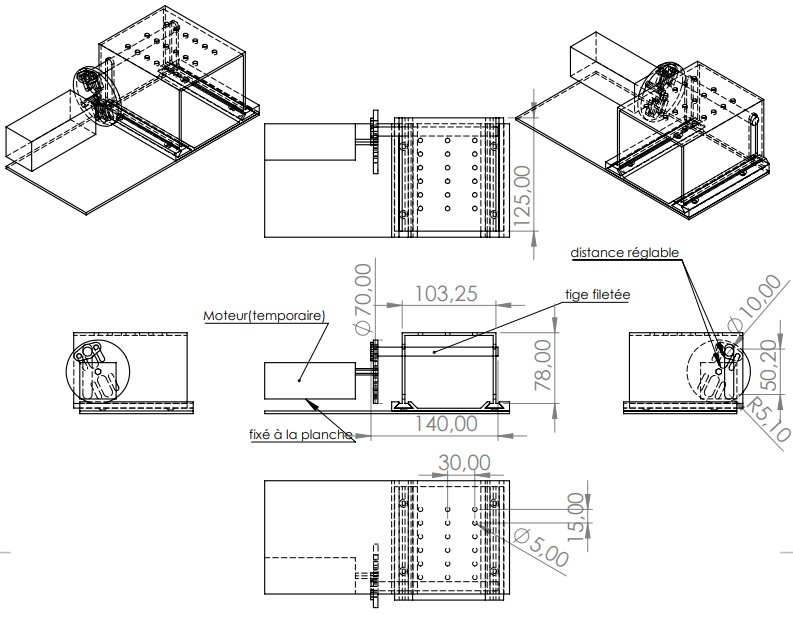
\includegraphics[width=0.9\textwidth]{C:/Users/noebo/OneDrive/Documents/Prépa/TIPE TMD/Présentation/Photos comp/sw axe linéaire-min.png}
				\caption{Planche solidworks du système vibratoire}
			\end{figure}
		\end{column}
	\end{columns}
\end{frame}

		\begin{frame}
			fonctionnement moteur pas à pas\\
			fonctionnement accéléromètre 
			
		\end{frame}
\end{document}